\SourceLeaf{215}\begin{center}
[3.]

PARALLELISMUS.
\end{center}

1. $ab\ast $ ist mit $cd\ast $ parallel, wenn

1) beide in einer Ebene sind,

2) einander nicht schneiden,

3) jede Linie $af\ast $ innerhalb des Raumes $\ast bacd\ast $ die $cd\ast $ schneidet.

\begin{center}
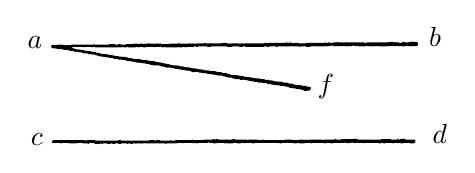
\begin{tikzpicture}[x=0.00583419cm,y=-0.00583419cm]
\fill[even odd rule] (875,255) -- (873,253) -- (854,253) -- (853,252) -- (850,252) -- (849,251) -- (847,251) -- (846,252) -- (842,252) -- (841,253) -- (839,253) -- (838,252) -- (835,252) -- (834,253) -- (822,253) -- (821,252) -- (801,252) -- (800,253) -- (789,253) -- (788,254) -- (786,253) -- (750,253) -- (749,252) -- (744,252) -- (743,251) -- (741,251) -- (740,252) -- (714,252) -- (713,253) -- (703,253) -- (702,252) -- (699,252) -- (698,253) -- (676,253) -- (675,254) -- (673,254) -- (672,253) -- (645,253) -- (644,254) -- (642,253) -- (640,254) -- (638,254) -- (637,253) -- (635,253) -- (634,254) -- (632,254) -- (631,253) -- (622,253) -- (621,254) -- (607,254) -- (606,253) -- (590,253) -- (589,254) -- (544,254) -- (543,253) -- (541,253) -- (540,254) -- (533,254) -- (532,253) -- (511,253) -- (510,254) -- (508,254) -- (507,253) -- (482,253) -- (481,252) -- (477,252) -- (476,253) -- (471,253) -- (469,254) -- (468,253) -- (446,253) -- (445,252) -- (441,252) -- (440,253) -- (438,253) -- (437,252) -- (434,252) -- (433,253) -- (426,253) -- (425,254) -- (423,253) -- (414,253) -- (413,254) -- (392,254) -- (391,253) -- (389,253) -- (388,254) -- (352,254) -- (351,255) -- (343,255) -- (342,254) -- (340,255) -- (319,255) -- (318,254) -- (311,254) -- (310,255) -- (307,255) -- (306,254) -- (295,254) -- (294,255) -- (234,255) -- (233,254) -- (228,254) -- (227,255) -- (177,255) -- (176,254) -- (160,254) -- (159,255) -- (156,255) -- (155,254) -- (86,254) -- (83,257) -- (83,259) -- (84,260) -- (100,260) -- (101,261) -- (104,261) -- (105,260) -- (119,260) -- (120,261) -- (137,261) -- (138,260) -- (149,260) -- (150,261) -- (160,261) -- (161,262) -- (163,262) -- (165,260) -- (173,260) -- (174,261) -- (176,261) -- (177,262) -- (181,262) -- (182,263) -- (184,262) -- (188,262) -- (189,261) -- (191,261) -- (192,262) -- (194,262) -- (195,261) -- (203,261) -- (204,262) -- (210,262) -- (211,261) -- (214,261) -- (215,262) -- (220,262) -- (221,261) -- (227,261) -- (228,262) -- (233,262) -- (234,261) -- (246,261) -- (247,262) -- (249,262) -- (250,261) -- (253,261) -- (254,262) -- (259,262) -- (260,261) -- (265,261) -- (266,262) -- (268,261) -- (275,261) -- (276,262) -- (278,261) -- (329,261) -- (330,262) -- (332,262) -- (333,261) -- (356,261) -- (357,260) -- (367,260) -- (368,261) -- (370,260) -- (390,260) -- (391,261) -- (397,260) -- (398,261) -- (401,261) -- (402,260) -- (422,260) -- (423,259) -- (425,259) -- (426,260) -- (433,260) -- (434,261) -- (441,261) -- (442,260) -- (457,260) -- (458,261) -- (461,261) -- (462,260) -- (464,261) -- (477,261) -- (478,260) -- (486,260) -- (487,261) -- (494,261) -- (495,260) -- (502,260) -- (503,261) -- (505,260) -- (518,260) -- (519,261) -- (524,261) -- (525,260) -- (575,260) -- (577,261) -- (579,260) -- (580,261) -- (583,261) -- (584,260) -- (594,260) -- (595,259) -- (597,260) -- (609,260) -- (610,261) -- (616,261) -- (617,260) -- (620,260) -- (621,261) -- (633,261) -- (634,260) -- (647,260) -- (648,261) -- (650,261) -- (651,260) -- (675,260) -- (676,261) -- (679,261) -- (680,260) -- (690,260) -- (691,261) -- (695,261) -- (696,260) -- (719,260) -- (720,259) -- (722,260) -- (727,260) -- (728,261) -- (730,260) -- (735,260) -- (736,259) -- (738,259) -- (739,260) -- (747,260) -- (749,259) -- (750,260) -- (762,260) -- (763,261) -- (765,260) -- (795,260) -- (796,261) -- (799,261) -- (800,260) -- (804,260) -- (805,261) -- (809,261) -- (810,260) -- (825,260) -- (826,261) -- (828,261) -- (829,260) -- (842,260) -- (843,261) -- (848,261) -- (849,260) -- (862,260) -- (863,261) -- (871,261) -- (875,259) -- cycle
(881,44) -- (880,42) -- (877,40) -- (870,40) -- (869,39) -- (867,40) -- (861,40) -- (860,41) -- (852,41) -- (851,40) -- (848,40) -- (845,42) -- (839,42) -- (838,41) -- (833,41) -- (832,40) -- (830,41) -- (827,41) -- (826,40) -- (821,40) -- (819,41) -- (817,40) -- (816,41) -- (770,41) -- (769,42) -- (764,42) -- (763,41) -- (719,41) -- (717,42) -- (716,41) -- (708,41) -- (706,40) -- (705,41) -- (696,41) -- (695,42) -- (688,42) -- (687,41) -- (685,41) -- (684,42) -- (680,42) -- (678,41) -- (677,42) -- (637,42) -- (636,43) -- (621,43) -- (620,42) -- (617,42) -- (616,43) -- (611,42) -- (610,43) -- (608,43) -- (607,42) -- (604,42) -- (603,41) -- (601,41) -- (600,42) -- (596,42) -- (595,41) -- (593,41) -- (592,42) -- (554,42) -- (553,43) -- (551,43) -- (550,42) -- (547,42) -- (546,43) -- (496,43) -- (495,44) -- (490,44) -- (489,43) -- (475,43) -- (474,44) -- (470,43) -- (469,44) -- (466,44) -- (464,42) -- (462,42) -- (461,43) -- (459,42) -- (457,43) -- (453,42) -- (452,43) -- (442,43) -- (441,44) -- (439,43) -- (426,43) -- (424,44) -- (423,43) -- (418,43) -- (416,42) -- (415,43) -- (402,43) -- (401,44) -- (392,44) -- (391,43) -- (389,44) -- (386,44) -- (385,43) -- (382,43) -- (381,44) -- (362,44) -- (361,43) -- (358,43) -- (357,44) -- (340,44) -- (339,45) -- (336,44) -- (335,45) -- (322,45) -- (319,43) -- (318,44) -- (313,44) -- (312,43) -- (310,44) -- (296,44) -- (295,43) -- (293,43) -- (292,44) -- (286,44) -- (285,45) -- (281,45) -- (280,44) -- (273,44) -- (272,45) -- (270,45) -- (269,44) -- (262,44) -- (261,45) -- (245,45) -- (244,46) -- (233,46) -- (232,45) -- (228,45) -- (227,46) -- (221,46) -- (220,45) -- (208,45) -- (207,46) -- (180,46) -- (179,47) -- (175,45) -- (174,46) -- (125,46) -- (124,47) -- (114,47) -- (113,48) -- (111,47) -- (108,47) -- (107,46) -- (96,46) -- (95,47) -- (88,47) -- (87,46) -- (85,46) -- (81,49) -- (81,51) -- (85,54) -- (92,54) -- (95,56) -- (100,55) -- (101,56) -- (106,56) -- (107,57) -- (120,58) -- (123,60) -- (131,60) -- (133,62) -- (138,61) -- (139,62) -- (142,62) -- (143,63) -- (148,63) -- (152,65) -- (160,65) -- (163,67) -- (165,67) -- (166,66) -- (168,66) -- (171,68) -- (175,67) -- (178,69) -- (184,70) -- (185,71) -- (188,71) -- (189,72) -- (195,72) -- (196,73) -- (207,74) -- (208,75) -- (215,75) -- (219,77) -- (226,77) -- (229,79) -- (234,78) -- (235,79) -- (244,80) -- (247,82) -- (255,82) -- (256,83) -- (261,83) -- (262,84) -- (266,84) -- (267,85) -- (275,85) -- (276,86) -- (281,86) -- (282,87) -- (287,87) -- (288,88) -- (294,88) -- (298,90) -- (303,90) -- (305,92) -- (307,91) -- (315,91) -- (316,92) -- (319,92) -- (322,94) -- (327,94) -- (328,95) -- (331,95) -- (332,96) -- (342,96) -- (343,97) -- (351,98) -- (352,99) -- (358,99) -- (359,100) -- (365,100) -- (366,101) -- (371,101) -- (372,102) -- (383,103) -- (384,104) -- (386,104) -- (388,106) -- (400,105) -- (404,107) -- (409,107) -- (410,108) -- (419,108) -- (422,110) -- (428,110) -- (429,111) -- (432,110) -- (433,111) -- (441,112) -- (442,113) -- (447,113) -- (448,114) -- (450,113) -- (453,113) -- (456,115) -- (460,115) -- (461,116) -- (467,117) -- (468,118) -- (475,118) -- (478,120) -- (482,120) -- (483,121) -- (491,121) -- (494,123) -- (498,123) -- (499,122) -- (501,122) -- (502,123) -- (506,123) -- (507,124) -- (511,124) -- (512,125) -- (518,125) -- (519,126) -- (523,126) -- (524,127) -- (530,127) -- (533,129) -- (537,129) -- (539,128) -- (542,130) -- (545,129) -- (546,130) -- (551,130) -- (554,132) -- (558,131) -- (561,133) -- (566,133) -- (567,134) -- (573,134) -- (574,135) -- (580,135) -- (581,136) -- (589,136) -- (590,137) -- (598,138) -- (601,140) -- (606,140) -- (609,142) -- (610,141) -- (613,141) -- (616,143) -- (624,143) -- (625,144) -- (631,145) -- (634,147) -- (638,147) -- (639,146) -- (644,146) -- (647,143) -- (647,140) -- (645,138) -- (641,138) -- (640,137) -- (636,137) -- (635,136) -- (629,136) -- (628,135) -- (625,135) -- (624,134) -- (614,134) -- (613,133) -- (610,133) -- (607,131) -- (600,131) -- (596,129) -- (588,129) -- (584,127) -- (568,126) -- (567,125) -- (564,125) -- (563,124) -- (557,124) -- (556,123) -- (548,123) -- (545,121) -- (538,121) -- (537,120) -- (522,119) -- (521,118) -- (516,118) -- (515,117) -- (508,117) -- (507,116) -- (502,116) -- (501,115) -- (491,114) -- (490,113) -- (473,112) -- (469,110) -- (465,110) -- (463,108) -- (455,108) -- (451,106) -- (444,106) -- (443,105) -- (440,105) -- (439,104) -- (431,104) -- (430,103) -- (425,103) -- (424,102) -- (415,102) -- (414,101) -- (411,101) -- (410,100) -- (403,100) -- (402,99) -- (397,99) -- (396,98) -- (389,98) -- (388,97) -- (385,97) -- (384,96) -- (372,95) -- (371,94) -- (361,93) -- (360,92) -- (356,92) -- (355,91) -- (346,91) -- (345,90) -- (340,90) -- (337,88) -- (331,88) -- (330,87) -- (326,87) -- (325,86) -- (321,86) -- (320,85) -- (311,84) -- (310,83) -- (307,83) -- (306,82) -- (297,82) -- (296,81) -- (291,81) -- (290,80) -- (282,80) -- (281,79) -- (278,79) -- (277,78) -- (260,77) -- (259,76) -- (249,75) -- (248,74) -- (245,74) -- (244,73) -- (229,72) -- (228,71) -- (222,71) -- (221,70) -- (216,70) -- (215,69) -- (209,69) -- (208,68) -- (204,68) -- (203,67) -- (190,66) -- (186,64) -- (181,64) -- (177,62) -- (172,62) -- (171,61) -- (168,61) -- (167,60) -- (160,60) -- (159,59) -- (153,59) -- (152,58) -- (148,58) -- (147,57) -- (134,56) -- (131,54) -- (128,54) -- (127,53) -- (128,51) -- (153,51) -- (154,52) -- (156,51) -- (170,51) -- (171,52) -- (173,51) -- (177,51) -- (178,52) -- (225,52) -- (226,51) -- (227,52) -- (228,51) -- (229,52) -- (235,52) -- (236,51) -- (238,51) -- (239,52) -- (245,52) -- (246,51) -- (248,51) -- (249,52) -- (265,52) -- (266,51) -- (269,51) -- (270,52) -- (272,52) -- (273,51) -- (281,51) -- (282,52) -- (287,52) -- (288,51) -- (305,51) -- (307,52) -- (308,51) -- (318,51) -- (320,50) -- (323,52) -- (326,52) -- (327,51) -- (329,51) -- (330,52) -- (357,52) -- (358,51) -- (360,51) -- (361,52) -- (365,52) -- (366,51) -- (372,51) -- (373,52) -- (375,52) -- (376,51) -- (392,51) -- (393,50) -- (397,50) -- (398,51) -- (400,51) -- (401,50) -- (421,50) -- (422,51) -- (429,51) -- (430,50) -- (464,50) -- (465,51) -- (475,51) -- (476,50) -- (491,50) -- (492,51) -- (498,51) -- (499,50) -- (504,50) -- (505,51) -- (526,51) -- (528,50) -- (529,51) -- (545,51) -- (546,50) -- (551,50) -- (552,51) -- (555,51) -- (556,50) -- (564,50) -- (565,49) -- (571,50) -- (572,51) -- (574,51) -- (575,50) -- (603,50) -- (604,49) -- (607,49) -- (608,50) -- (622,50) -- (623,51) -- (625,50) -- (632,50) -- (634,49) -- (638,51) -- (644,51) -- (645,50) -- (651,50) -- (652,49) -- (656,49) -- (657,50) -- (659,49) -- (661,50) -- (675,50) -- (676,49) -- (678,49) -- (679,50) -- (681,50) -- (682,49) -- (689,49) -- (690,48) -- (696,48) -- (698,50) -- (700,50) -- (701,49) -- (724,49) -- (725,50) -- (727,50) -- (728,49) -- (737,49) -- (738,48) -- (742,48) -- (743,49) -- (747,49) -- (749,48) -- (752,50) -- (755,50) -- (756,49) -- (758,49) -- (759,50) -- (764,50) -- (765,49) -- (776,49) -- (777,50) -- (779,50) -- (780,49) -- (782,50) -- (784,50) -- (785,49) -- (796,49) -- (797,50) -- (812,50) -- (813,49) -- (845,49) -- (846,50) -- (850,50) -- (851,49) -- (878,49) -- (880,47) -- cycle;
\node[inner sep=0pt] at (918,30) {$b$};
\node[inner sep=0pt] at (46,41) {$a$};
\node[inner sep=0pt] at (680,138) {$f$};
\node[inner sep=0pt] at (928,240) {$d$};
\node[inner sep=0pt] at (50,252) {$c$};
\end{tikzpicture}

\end{center}

2. Der Parallelismus ist unabhängig von dem Anfang der Linie $cd\ast $.

3. Der Parallelismus ist unabhängig von dem Anfang der Linie $ab\ast $.

I. Es ist auch $a'b\ast $ parallel mit $cd\ast $, wenn $a'$ auf $ab\ast $.

\textls{Beweis.} $af\ast $ schneidet $cd\ast $; so wird auch $a'f\ast $ schneiden.

\Needspace{12\baselineskip}
II. [Es ist auch $a'b\ast $ parallel mit $cd\ast $,] wenn $a'$ ausserhalb $ab\ast $.

\begin{center}
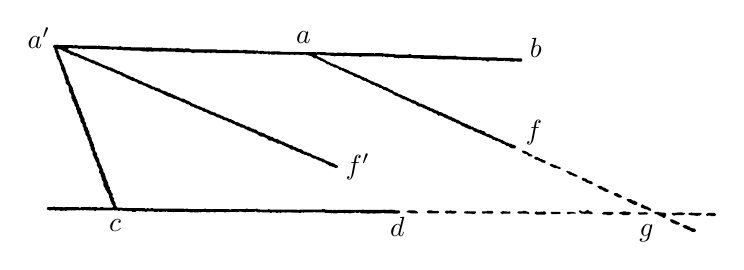
\begin{tikzpicture}[x=0.00597898cm,y=-0.00597898cm]
\fill[even odd rule] (1429,448) -- (1429,449) -- (1433,453) -- (1437,454) -- (1440,456) -- (1442,456) -- (1448,460) -- (1453,461) -- (1457,459) -- (1457,457) -- (1455,454) -- (1453,453) -- (1450,453) -- (1449,452) -- (1446,452) -- (1443,449) -- (1441,449) -- (1436,446) -- (1432,446) -- cycle
(1402,435) -- (1403,438) -- (1406,441) -- (1410,443) -- (1412,443) -- (1415,445) -- (1421,445) -- (1423,443) -- (1423,442) -- (1421,440) -- (1419,440) -- (1415,437) -- (1411,436) -- (1408,434) -- (1403,434) -- cycle
(1479,423) -- (1479,425) -- (1481,427) -- (1483,426) -- (1488,426) -- (1489,427) -- (1497,427) -- (1500,424) -- (1500,423) -- (1496,420) -- (1483,420) -- cycle
(1441,422) -- (1441,423) -- (1444,425) -- (1458,426) -- (1459,427) -- (1461,426) -- (1465,426) -- (1469,423) -- (1469,421) -- (1468,420) -- (1449,420) -- (1448,419) -- (1446,420) -- (1443,420) -- cycle
(1406,421) -- (1406,423) -- (1410,426) -- (1412,426) -- (1413,425) -- (1430,425) -- (1434,422) -- (1433,420) -- (1429,420) -- (1428,419) -- (1421,419) -- (1420,420) -- (1417,419) -- (1416,420) -- (1407,420) -- cycle
(1369,420) -- (1369,421) -- (1371,423) -- (1374,423) -- (1383,428) -- (1385,428) -- (1388,431) -- (1390,431) -- (1392,429) -- (1394,425) -- (1394,422) -- (1392,420) -- (1379,419) -- (1378,418) -- (1371,418) -- cycle
(1355,421) -- (1353,419) -- (1350,419) -- (1349,418) -- (1347,419) -- (1335,419) -- (1334,420) -- (1334,422) -- (1337,424) -- (1348,424) -- (1349,423) -- (1352,424) -- (1354,423) -- cycle
(1258,421) -- (1258,422) -- (1261,424) -- (1264,424) -- (1266,423) -- (1269,425) -- (1276,425) -- (1282,422) -- (1282,420) -- (1280,418) -- (1262,418) -- cycle
(1183,420) -- (1183,421) -- (1185,423) -- (1189,423) -- (1190,422) -- (1201,422) -- (1202,421) -- (1201,419) -- (1198,419) -- (1197,418) -- (1185,418) -- cycle
(1149,419) -- (1149,421) -- (1151,423) -- (1162,423) -- (1163,422) -- (1168,423) -- (1170,421) -- (1170,420) -- (1168,418) -- (1150,418) -- cycle
(1294,420) -- (1294,421) -- (1296,423) -- (1299,423) -- (1302,425) -- (1314,425) -- (1319,421) -- (1319,420) -- (1316,418) -- (1309,418) -- (1308,417) -- (1302,417) -- (1301,418) -- (1298,418) -- cycle
(1115,419) -- (1115,422) -- (1119,424) -- (1136,424) -- (1139,422) -- (1139,420) -- (1136,417) -- (1133,417) -- (1132,418) -- (1130,418) -- (1129,417) -- (1127,418) -- (1121,418) -- (1119,417) -- cycle
(1078,419) -- (1079,421) -- (1081,421) -- (1082,422) -- (1087,422) -- (1088,421) -- (1090,422) -- (1099,422) -- (1100,423) -- (1102,423) -- (1103,422) -- (1103,420) -- (1101,418) -- (1097,417) -- (1096,416) -- (1090,416) -- (1089,417) -- (1080,417) -- cycle
(1042,419) -- (1042,420) -- (1046,423) -- (1048,422) -- (1062,422) -- (1063,421) -- (1063,418) -- (1062,417) -- (1056,418) -- (1055,417) -- (1050,417) -- (1048,416) -- cycle
(1003,418) -- (1003,420) -- (1005,422) -- (1008,422) -- (1009,421) -- (1014,421) -- (1015,422) -- (1024,422) -- (1027,420) -- (1025,416) -- (1020,416) -- (1019,417) -- (1017,416) -- (1014,416) -- (1013,417) -- (1004,417) -- cycle
(965,419) -- (966,421) -- (968,421) -- (969,422) -- (981,422) -- (982,423) -- (988,422) -- (990,420) -- (990,418) -- (989,417) -- (973,417) -- (972,416) -- (970,417) -- (967,417) -- cycle
(924,418) -- (924,419) -- (928,422) -- (930,422) -- (931,421) -- (944,422) -- (949,419) -- (949,418) -- (947,416) -- (939,416) -- (938,415) -- (934,415) -- (933,416) -- (928,415) -- cycle
(886,417) -- (886,419) -- (889,421) -- (909,421) -- (912,419) -- (912,418) -- (909,416) -- (898,416) -- (897,415) -- (889,415) -- cycle
(843,417) -- (844,419) -- (850,420) -- (851,421) -- (866,421) -- (867,420) -- (867,419) -- (864,416) -- (862,416) -- (861,415) -- (847,415) -- cycle
(1238,421) -- (1238,420) -- (1236,418) -- (1234,417) -- (1231,417) -- (1228,414) -- (1226,414) -- (1224,416) -- (1220,418) -- (1214,417) -- (1212,415) -- (1210,415) -- (1209,416) -- (1209,418) -- (1214,422) -- (1220,422) -- (1221,423) -- (1223,422) -- (1231,422) -- (1232,423) -- (1236,423) -- cycle
(1340,405) -- (1340,408) -- (1343,410) -- (1345,410) -- (1348,412) -- (1354,413) -- (1356,415) -- (1358,415) -- (1359,416) -- (1360,416) -- (1362,414) -- (1360,410) -- (1357,409) -- (1355,407) -- (1350,406) -- (1344,402) -- (1343,402) -- cycle
(1310,392) -- (1310,393) -- (1314,397) -- (1326,403) -- (1331,403) -- (1333,400) -- (1333,398) -- (1326,394) -- (1323,394) -- (1319,391) -- (1311,391) -- cycle
(1283,380) -- (1283,382) -- (1284,383) -- (1294,388) -- (1298,388) -- (1300,386) -- (1300,385) -- (1297,382) -- (1294,381) -- (1290,378) -- (1285,378) -- cycle
(1248,364) -- (1248,365) -- (1253,370) -- (1256,370) -- (1264,375) -- (1269,376) -- (1272,374) -- (1272,372) -- (1270,370) -- (1268,370) -- (1264,367) -- (1260,366) -- (1256,363) -- (1249,363) -- cycle
(1215,347) -- (1215,350) -- (1217,352) -- (1222,353) -- (1224,355) -- (1228,357) -- (1230,357) -- (1232,359) -- (1237,359) -- (1238,358) -- (1238,356) -- (1235,353) -- (1228,351) -- (1224,347) -- (1220,347) -- (1219,346) -- (1216,346) -- cycle
(1182,332) -- (1182,333) -- (1189,339) -- (1194,340) -- (1200,343) -- (1205,343) -- (1206,342) -- (1205,340) -- (1197,336) -- (1195,336) -- (1193,334) -- (1189,332) -- (1186,332) -- (1185,331) -- (1183,331) -- cycle
(1147,318) -- (1147,319) -- (1149,321) -- (1157,325) -- (1162,325) -- (1166,327) -- (1169,327) -- (1170,326) -- (1170,324) -- (1167,322) -- (1164,322) -- (1162,320) -- (1160,320) -- (1158,318) -- (1155,318) -- (1152,316) -- (1149,316) -- cycle
(1114,303) -- (1114,305) -- (1118,308) -- (1121,307) -- (1124,310) -- (1126,310) -- (1130,313) -- (1136,314) -- (1138,312) -- (1138,310) -- (1137,309) -- (1133,308) -- (1130,306) -- (1128,306) -- (1120,301) -- (1116,301) -- cycle
(1088,289) -- (1088,291) -- (1090,293) -- (1094,295) -- (1098,295) -- (1102,300) -- (1109,300) -- (1110,299) -- (1110,298) -- (1108,296) -- (1103,294) -- (1101,292) -- (1095,289) -- (1093,289) -- (1092,288) -- (1089,288) -- cycle
(92,66) -- (93,69) -- (95,71) -- (95,74) -- (96,75) -- (97,80) -- (99,83) -- (99,88) -- (101,90) -- (101,93) -- (104,96) -- (104,98) -- (106,101) -- (106,103) -- (109,110) -- (109,114) -- (114,124) -- (114,126) -- (116,130) -- (116,133) -- (119,140) -- (119,145) -- (125,151) -- (126,161) -- (127,162) -- (127,164) -- (129,166) -- (131,170) -- (131,177) -- (133,179) -- (133,182) -- (135,184) -- (138,190) -- (138,193) -- (141,196) -- (141,200) -- (143,203) -- (144,209) -- (147,212) -- (148,218) -- (150,220) -- (150,225) -- (152,229) -- (155,232) -- (155,237) -- (157,239) -- (157,243) -- (161,250) -- (161,254) -- (165,259) -- (165,263) -- (168,268) -- (168,270) -- (170,274) -- (170,278) -- (172,280) -- (172,284) -- (174,288) -- (176,290) -- (176,297) -- (178,299) -- (178,301) -- (182,308) -- (182,310) -- (185,314) -- (185,319) -- (191,329) -- (190,331) -- (190,335) -- (193,338) -- (194,344) -- (195,345) -- (195,348) -- (197,352) -- (199,354) -- (199,362) -- (203,369) -- (203,371) -- (206,374) -- (207,377) -- (209,379) -- (211,383) -- (211,387) -- (213,390) -- (214,395) -- (216,397) -- (216,400) -- (219,404) -- (220,407) -- (218,409) -- (199,409) -- (198,408) -- (193,408) -- (192,409) -- (186,409) -- (185,408) -- (175,408) -- (173,409) -- (170,407) -- (168,408) -- (152,408) -- (151,409) -- (147,409) -- (146,408) -- (117,408) -- (115,409) -- (114,408) -- (97,408) -- (96,407) -- (93,407) -- (92,408) -- (81,408) -- (79,410) -- (79,412) -- (81,414) -- (83,414) -- (84,415) -- (95,414) -- (98,416) -- (99,415) -- (107,415) -- (108,416) -- (117,415) -- (118,416) -- (120,416) -- (121,415) -- (141,415) -- (142,414) -- (144,414) -- (145,415) -- (148,415) -- (149,414) -- (157,415) -- (158,414) -- (162,414) -- (163,415) -- (179,415) -- (180,416) -- (182,416) -- (183,415) -- (218,415) -- (219,414) -- (221,414) -- (222,415) -- (230,415) -- (231,416) -- (233,416) -- (234,415) -- (239,415) -- (240,416) -- (249,416) -- (250,417) -- (258,416) -- (260,418) -- (267,418) -- (269,416) -- (274,416) -- (275,417) -- (280,416) -- (281,417) -- (287,417) -- (288,418) -- (290,418) -- (291,417) -- (306,417) -- (307,418) -- (314,418) -- (315,417) -- (317,417) -- (318,418) -- (324,418) -- (325,417) -- (331,418) -- (332,417) -- (334,417) -- (335,418) -- (347,418) -- (348,419) -- (350,418) -- (373,418) -- (374,417) -- (376,418) -- (382,418) -- (383,419) -- (389,419) -- (390,418) -- (392,419) -- (401,419) -- (402,418) -- (404,419) -- (406,419) -- (407,418) -- (417,418) -- (418,419) -- (420,419) -- (421,418) -- (423,419) -- (425,419) -- (426,418) -- (432,418) -- (433,419) -- (437,419) -- (438,418) -- (454,418) -- (455,419) -- (460,419) -- (461,418) -- (464,418) -- (465,419) -- (467,418) -- (481,418) -- (483,419) -- (484,418) -- (487,418) -- (488,417) -- (501,419) -- (502,418) -- (520,418) -- (521,417) -- (523,417) -- (527,419) -- (531,419) -- (532,418) -- (534,418) -- (535,419) -- (552,419) -- (553,420) -- (556,420) -- (557,419) -- (565,419) -- (566,420) -- (570,420) -- (571,419) -- (573,419) -- (574,420) -- (576,420) -- (577,419) -- (585,419) -- (586,420) -- (588,419) -- (618,420) -- (619,419) -- (622,419) -- (624,420) -- (625,419) -- (645,419) -- (646,418) -- (648,418) -- (649,419) -- (669,419) -- (670,420) -- (681,420) -- (682,421) -- (684,421) -- (685,420) -- (687,421) -- (695,421) -- (696,420) -- (709,420) -- (710,421) -- (712,421) -- (713,420) -- (719,420) -- (720,421) -- (725,421) -- (726,420) -- (731,420) -- (732,419) -- (735,419) -- (736,420) -- (741,420) -- (742,419) -- (744,419) -- (746,421) -- (758,421) -- (759,422) -- (764,422) -- (765,421) -- (772,421) -- (773,422) -- (776,422) -- (777,421) -- (789,421) -- (790,420) -- (794,420) -- (795,421) -- (813,421) -- (814,422) -- (823,422) -- (824,421) -- (827,421) -- (829,419) -- (829,417) -- (827,415) -- (819,415) -- (818,414) -- (813,414) -- (812,413) -- (810,413) -- (809,414) -- (807,414) -- (806,413) -- (804,414) -- (797,414) -- (796,413) -- (794,413) -- (793,414) -- (752,414) -- (751,413) -- (749,413) -- (748,414) -- (696,414) -- (695,415) -- (693,414) -- (687,414) -- (685,415) -- (684,414) -- (674,414) -- (673,413) -- (670,413) -- (669,412) -- (664,412) -- (663,413) -- (617,413) -- (616,414) -- (611,414) -- (610,413) -- (552,413) -- (550,412) -- (549,413) -- (544,413) -- (542,414) -- (541,413) -- (531,413) -- (530,412) -- (528,413) -- (525,411) -- (523,411) -- (522,412) -- (506,412) -- (505,411) -- (502,411) -- (501,412) -- (471,412) -- (470,413) -- (467,413) -- (466,412) -- (429,412) -- (427,413) -- (426,412) -- (417,412) -- (416,411) -- (414,411) -- (413,412) -- (379,412) -- (378,411) -- (374,411) -- (373,412) -- (371,412) -- (370,411) -- (305,411) -- (304,410) -- (300,410) -- (299,411) -- (295,411) -- (294,410) -- (292,410) -- (291,411) -- (288,411) -- (287,410) -- (248,410) -- (247,409) -- (245,410) -- (240,410) -- (239,409) -- (229,409) -- (225,404) -- (225,400) -- (221,393) -- (222,390) -- (218,385) -- (219,380) -- (216,377) -- (215,373) -- (213,371) -- (213,366) -- (210,363) -- (210,361) -- (209,360) -- (209,355) -- (207,353) -- (207,351) -- (205,349) -- (205,347) -- (204,346) -- (204,342) -- (202,340) -- (202,337) -- (199,333) -- (198,327) -- (196,325) -- (195,320) -- (191,313) -- (190,306) -- (186,300) -- (185,293) -- (183,291) -- (181,287) -- (181,283) -- (179,279) -- (179,275) -- (177,272) -- (177,270) -- (175,268) -- (175,266) -- (174,265) -- (174,261) -- (172,259) -- (172,256) -- (169,252) -- (169,247) -- (166,243) -- (166,240) -- (163,237) -- (162,229) -- (159,226) -- (159,221) -- (154,211) -- (154,207) -- (151,203) -- (151,199) -- (148,196) -- (148,193) -- (147,192) -- (147,190) -- (145,188) -- (144,182) -- (141,177) -- (141,175) -- (137,167) -- (137,165) -- (136,164) -- (136,160) -- (134,158) -- (134,155) -- (128,144) -- (128,142) -- (126,140) -- (126,138) -- (125,137) -- (125,132) -- (120,122) -- (120,119) -- (119,118) -- (118,113) -- (116,110) -- (116,108) -- (114,104) -- (112,102) -- (111,96) -- (108,92) -- (108,89) -- (104,81) -- (104,77) -- (102,75) -- (102,73) -- (104,71) -- (106,73) -- (108,73) -- (112,75) -- (114,77) -- (117,77) -- (121,80) -- (126,81) -- (130,85) -- (135,85) -- (137,87) -- (139,87) -- (140,88) -- (144,88) -- (146,90) -- (150,92) -- (155,93) -- (161,97) -- (164,97) -- (176,103) -- (180,103) -- (183,106) -- (185,107) -- (188,107) -- (191,109) -- (193,109) -- (200,113) -- (202,113) -- (206,115) -- (208,117) -- (212,117) -- (217,120) -- (220,120) -- (222,122) -- (226,123) -- (228,125) -- (234,126) -- (241,131) -- (244,131) -- (249,135) -- (251,135) -- (261,140) -- (266,141) -- (272,144) -- (274,146) -- (282,148) -- (284,150) -- (286,150) -- (302,158) -- (306,158) -- (309,161) -- (315,162) -- (317,164) -- (319,164) -- (336,173) -- (341,174) -- (349,178) -- (352,178) -- (356,180) -- (359,180) -- (361,182) -- (369,186) -- (372,186) -- (377,190) -- (381,190) -- (385,194) -- (391,195) -- (393,197) -- (395,197) -- (397,199) -- (400,199) -- (403,201) -- (408,202) -- (411,205) -- (417,206) -- (425,211) -- (433,213) -- (442,218) -- (445,218) -- (448,220) -- (450,220) -- (454,223) -- (460,224) -- (466,228) -- (469,228) -- (474,231) -- (476,231) -- (482,235) -- (489,237) -- (491,239) -- (496,239) -- (500,242) -- (503,243) -- (505,245) -- (507,245) -- (510,247) -- (513,247) -- (515,249) -- (518,249) -- (521,251) -- (525,252) -- (528,255) -- (533,258) -- (538,258) -- (546,262) -- (551,267) -- (558,267) -- (560,269) -- (562,269) -- (566,271) -- (568,273) -- (574,273) -- (575,274) -- (577,274) -- (579,276) -- (593,282) -- (598,286) -- (603,286) -- (612,291) -- (615,291) -- (617,293) -- (619,293) -- (621,295) -- (623,295) -- (627,297) -- (630,297) -- (633,299) -- (638,300) -- (640,302) -- (646,305) -- (650,305) -- (652,307) -- (654,307) -- (656,309) -- (659,309) -- (661,311) -- (663,311) -- (665,313) -- (668,313) -- (670,314) -- (673,317) -- (675,317) -- (680,321) -- (683,321) -- (684,322) -- (689,323) -- (691,325) -- (696,324) -- (697,323) -- (697,321) -- (695,319) -- (693,319) -- (691,317) -- (685,314) -- (683,314) -- (677,311) -- (675,311) -- (673,309) -- (671,309) -- (665,305) -- (660,304) -- (655,301) -- (652,301) -- (650,299) -- (644,298) -- (639,294) -- (637,294) -- (634,292) -- (631,292) -- (629,290) -- (625,290) -- (622,287) -- (618,285) -- (615,285) -- (606,280) -- (603,280) -- (600,277) -- (594,276) -- (590,273) -- (588,273) -- (581,269) -- (578,269) -- (576,267) -- (574,267) -- (570,264) -- (563,263) -- (558,259) -- (555,259) -- (552,257) -- (545,255) -- (540,251) -- (537,251) -- (534,249) -- (531,249) -- (527,247) -- (524,244) -- (522,243) -- (519,243) -- (517,241) -- (514,241) -- (512,239) -- (510,239) -- (508,237) -- (503,237) -- (499,234) -- (495,233) -- (493,231) -- (490,231) -- (485,228) -- (479,227) -- (477,225) -- (469,221) -- (467,221) -- (461,218) -- (458,218) -- (452,214) -- (450,214) -- (445,211) -- (442,211) -- (438,209) -- (436,207) -- (433,207) -- (430,205) -- (428,205) -- (421,201) -- (419,201) -- (415,199) -- (413,197) -- (410,197) -- (404,194) -- (399,193) -- (397,191) -- (390,189) -- (386,187) -- (384,185) -- (378,182) -- (374,181) -- (371,178) -- (363,177) -- (359,174) -- (356,174) -- (353,171) -- (351,171) -- (345,168) -- (343,168) -- (341,166) -- (336,165) -- (334,163) -- (323,160) -- (318,156) -- (315,156) -- (314,155) -- (309,154) -- (306,152) -- (303,152) -- (301,150) -- (297,148) -- (295,148) -- (293,146) -- (288,145) -- (282,142) -- (280,140) -- (277,140) -- (274,138) -- (272,138) -- (270,136) -- (267,136) -- (265,134) -- (261,132) -- (259,132) -- (252,128) -- (250,128) -- (242,124) -- (240,122) -- (235,121) -- (233,119) -- (230,119) -- (214,111) -- (211,111) -- (206,108) -- (203,108) -- (200,106) -- (198,106) -- (196,104) -- (192,103) -- (186,99) -- (183,99) -- (181,97) -- (170,94) -- (168,92) -- (165,92) -- (163,90) -- (159,89) -- (156,87) -- (154,87) -- (147,83) -- (145,83) -- (143,81) -- (139,81) -- (132,77) -- (130,77) -- (128,75) -- (126,75) -- (124,73) -- (124,72) -- (126,70) -- (131,70) -- (132,71) -- (145,71) -- (146,72) -- (153,71) -- (157,73) -- (161,72) -- (162,71) -- (164,72) -- (178,72) -- (179,73) -- (181,72) -- (191,72) -- (192,73) -- (208,73) -- (209,74) -- (210,73) -- (217,73) -- (218,74) -- (220,74) -- (221,73) -- (227,73) -- (228,74) -- (240,74) -- (241,75) -- (281,76) -- (282,77) -- (290,77) -- (291,78) -- (295,78) -- (296,77) -- (300,77) -- (301,78) -- (305,78) -- (306,77) -- (317,77) -- (318,78) -- (322,78) -- (323,77) -- (331,77) -- (332,78) -- (348,78) -- (350,77) -- (353,79) -- (369,79) -- (370,80) -- (372,79) -- (384,79) -- (385,80) -- (388,80) -- (389,81) -- (391,81) -- (392,80) -- (413,80) -- (414,81) -- (418,81) -- (419,80) -- (425,80) -- (426,81) -- (428,81) -- (429,80) -- (437,80) -- (438,81) -- (447,81) -- (449,80) -- (450,81) -- (499,81) -- (500,82) -- (518,82) -- (519,83) -- (527,81) -- (528,82) -- (531,82) -- (532,83) -- (535,83) -- (536,82) -- (538,82) -- (539,83) -- (548,82) -- (550,84) -- (552,84) -- (553,83) -- (555,83) -- (556,84) -- (564,84) -- (565,83) -- (567,83) -- (568,84) -- (593,84) -- (594,85) -- (596,84) -- (603,84) -- (604,85) -- (606,85) -- (607,84) -- (615,84) -- (616,85) -- (629,84) -- (630,85) -- (634,85) -- (635,86) -- (640,87) -- (647,92) -- (652,92) -- (660,97) -- (665,98) -- (667,100) -- (669,100) -- (674,105) -- (678,105) -- (682,108) -- (684,108) -- (691,112) -- (694,112) -- (698,114) -- (701,117) -- (705,117) -- (707,119) -- (709,119) -- (713,122) -- (718,123) -- (720,125) -- (727,127) -- (732,131) -- (737,132) -- (740,134) -- (743,134) -- (750,139) -- (756,140) -- (758,142) -- (762,143) -- (770,148) -- (775,149) -- (779,152) -- (782,152) -- (786,155) -- (789,155) -- (794,159) -- (797,159) -- (800,161) -- (802,161) -- (806,164) -- (812,166) -- (818,171) -- (825,173) -- (836,179) -- (839,179) -- (843,181) -- (845,183) -- (848,183) -- (856,188) -- (860,188) -- (867,194) -- (875,195) -- (879,198) -- (881,198) -- (883,200) -- (885,200) -- (892,204) -- (895,204) -- (899,207) -- (903,209) -- (905,209) -- (911,214) -- (913,213) -- (917,214) -- (921,216) -- (923,218) -- (925,218) -- (928,220) -- (930,220) -- (932,222) -- (934,222) -- (938,224) -- (940,226) -- (943,226) -- (944,227) -- (946,227) -- (949,230) -- (955,231) -- (961,236) -- (965,237) -- (967,239) -- (969,239) -- (977,243) -- (982,243) -- (988,248) -- (990,248) -- (996,251) -- (998,251) -- (1005,255) -- (1012,257) -- (1014,259) -- (1017,259) -- (1019,261) -- (1022,261) -- (1025,264) -- (1027,265) -- (1030,265) -- (1032,267) -- (1037,268) -- (1043,271) -- (1045,273) -- (1050,274) -- (1055,278) -- (1059,278) -- (1062,281) -- (1066,283) -- (1073,283) -- (1075,280) -- (1075,279) -- (1073,277) -- (1069,275) -- (1067,275) -- (1064,273) -- (1060,273) -- (1058,271) -- (1055,271) -- (1045,265) -- (1043,265) -- (1040,263) -- (1038,263) -- (1035,261) -- (1028,259) -- (1026,257) -- (1018,253) -- (1015,253) -- (1011,251) -- (1008,247) -- (1003,246) -- (1000,244) -- (996,244) -- (995,243) -- (993,243) -- (991,241) -- (987,240) -- (983,237) -- (980,237) -- (978,235) -- (976,235) -- (970,231) -- (967,231) -- (964,229) -- (962,229) -- (958,227) -- (956,225) -- (950,222) -- (948,222) -- (944,219) -- (940,218) -- (938,216) -- (935,216) -- (924,210) -- (922,210) -- (918,207) -- (912,206) -- (909,203) -- (906,203) -- (897,198) -- (894,198) -- (892,196) -- (888,195) -- (879,190) -- (876,190) -- (874,188) -- (870,188) -- (867,185) -- (865,185) -- (862,182) -- (859,182) -- (858,181) -- (853,180) -- (851,178) -- (849,178) -- (847,176) -- (845,176) -- (843,174) -- (840,174) -- (838,172) -- (836,172) -- (831,169) -- (826,168) -- (822,165) -- (817,164) -- (813,160) -- (809,159) -- (799,153) -- (796,153) -- (790,150) -- (788,148) -- (786,148) -- (783,146) -- (776,144) -- (771,141) -- (769,141) -- (759,136) -- (757,134) -- (754,134) -- (752,132) -- (750,132) -- (741,127) -- (739,127) -- (731,123) -- (729,123) -- (727,121) -- (725,121) -- (721,119) -- (719,117) -- (716,117) -- (714,115) -- (712,115) -- (709,113) -- (706,113) -- (691,105) -- (688,105) -- (686,103) -- (683,103) -- (679,100) -- (673,98) -- (670,95) -- (666,94) -- (664,92) -- (662,92) -- (660,90) -- (658,90) -- (654,88) -- (652,86) -- (652,85) -- (653,84) -- (659,84) -- (660,85) -- (681,86) -- (682,87) -- (688,87) -- (689,88) -- (691,88) -- (692,87) -- (707,87) -- (708,88) -- (710,88) -- (711,87) -- (724,87) -- (725,88) -- (742,88) -- (743,89) -- (746,89) -- (747,88) -- (790,88) -- (791,89) -- (793,88) -- (796,88) -- (797,89) -- (800,89) -- (801,90) -- (803,90) -- (804,89) -- (814,89) -- (817,91) -- (824,91) -- (825,92) -- (827,92) -- (828,91) -- (833,91) -- (834,92) -- (836,91) -- (856,91) -- (857,92) -- (872,92) -- (873,93) -- (907,93) -- (908,94) -- (921,94) -- (922,95) -- (924,94) -- (942,94) -- (943,95) -- (945,94) -- (948,94) -- (949,95) -- (957,94) -- (958,95) -- (962,95) -- (963,96) -- (965,95) -- (967,96) -- (971,96) -- (972,95) -- (974,95) -- (975,96) -- (1002,96) -- (1003,97) -- (1007,97) -- (1009,96) -- (1015,99) -- (1016,99) -- (1018,97) -- (1034,97) -- (1035,98) -- (1052,97) -- (1053,98) -- (1062,98) -- (1063,99) -- (1072,99) -- (1073,98) -- (1076,98) -- (1077,99) -- (1087,99) -- (1088,98) -- (1088,94) -- (1086,92) -- (1069,92) -- (1068,91) -- (1036,91) -- (1035,90) -- (1000,90) -- (999,89) -- (997,90) -- (993,90) -- (992,89) -- (982,89) -- (980,90) -- (979,89) -- (949,88) -- (946,86) -- (944,87) -- (916,87) -- (915,86) -- (909,87) -- (908,86) -- (854,85) -- (851,83) -- (848,83) -- (847,84) -- (819,84) -- (818,83) -- (806,83) -- (805,82) -- (794,82) -- (793,81) -- (776,81) -- (775,82) -- (773,81) -- (724,81) -- (723,80) -- (721,81) -- (717,81) -- (716,80) -- (709,80) -- (708,81) -- (704,81) -- (703,80) -- (695,80) -- (694,81) -- (690,81) -- (689,80) -- (672,80) -- (671,79) -- (653,79) -- (651,80) -- (650,79) -- (574,78) -- (573,77) -- (556,77) -- (555,78) -- (553,78) -- (552,77) -- (540,77) -- (539,76) -- (531,76) -- (530,77) -- (528,77) -- (526,75) -- (521,76) -- (520,75) -- (505,75) -- (504,74) -- (496,74) -- (495,75) -- (487,75) -- (486,74) -- (472,74) -- (471,75) -- (469,75) -- (468,74) -- (440,74) -- (439,73) -- (385,73) -- (381,71) -- (372,71) -- (371,72) -- (369,72) -- (368,71) -- (359,71) -- (358,70) -- (355,70) -- (354,71) -- (343,71) -- (342,70) -- (340,70) -- (339,71) -- (335,71) -- (334,70) -- (325,70) -- (324,69) -- (322,70) -- (303,70) -- (302,69) -- (290,69) -- (288,70) -- (287,69) -- (258,69) -- (257,68) -- (243,68) -- (241,69) -- (239,67) -- (237,67) -- (236,66) -- (234,66) -- (233,67) -- (213,67) -- (211,66) -- (209,67) -- (208,66) -- (197,66) -- (196,65) -- (194,66) -- (192,66) -- (191,65) -- (188,65) -- (187,66) -- (185,66) -- (184,65) -- (144,65) -- (143,64) -- (138,64) -- (137,65) -- (135,65) -- (134,64) -- (103,64) -- (102,63) -- (100,63) -- (99,64) -- (95,63) -- cycle;
\node[inner sep=0pt] at (62,49) {$a'$};
\node[inner sep=0pt] at (624,47) {$a$};
\node[inner sep=0pt] at (1117,70) {$b$};
\node[inner sep=0pt] at (1113,250) {$f$};
\node[inner sep=0pt] at (739,323) {$f'$};
\node[inner sep=0pt] at (823,450) {$d$};
\node[inner sep=0pt] at (224,447) {$c$};
\node[inner sep=0pt] at (1352,464) {$g$};
\end{tikzpicture}

\end{center}

Man mache $baf = ba'f'$; es schneide $af\ast $ die $cd\ast $ in $g$, so wird $a'f'$ die $af\ast $ nicht schneiden, also $cg$.

4. Es ist verstattet $ab\ast $ und $cd\ast $ zu vertauschen.

\begin{center}
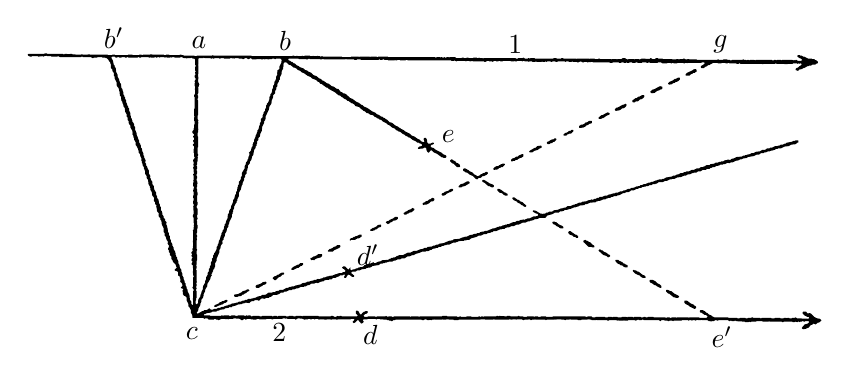
\begin{tikzpicture}[x=0.00604106cm,y=-0.00604106cm]
\fill[even odd rule] (1401,598) -- (1401,601) -- (1404,604) -- (1410,607) -- (1412,609) -- (1422,614) -- (1424,614) -- (1426,612) -- (1426,610) -- (1424,608) -- (1423,608) -- (1420,605) -- (1415,603) -- (1407,597) -- (1402,597) -- cycle
(441,597) -- (439,595) -- (438,595) -- (432,598) -- (430,598) -- (427,600) -- (425,600) -- (422,603) -- (415,606) -- (413,608) -- (413,609) -- (414,610) -- (417,610) -- (423,607) -- (425,607) -- (428,605) -- (430,605) -- (434,602) -- (438,601) -- (441,598) -- cycle
(1363,575) -- (1363,578) -- (1367,582) -- (1369,582) -- (1379,590) -- (1382,590) -- (1383,591) -- (1388,591) -- (1390,589) -- (1390,588) -- (1388,586) -- (1380,582) -- (1374,577) -- (1372,577) -- (1366,574) -- (1364,574) -- cycle
(487,575) -- (485,573) -- (482,573) -- (480,575) -- (473,577) -- (471,579) -- (463,583) -- (456,584) -- (455,585) -- (455,587) -- (457,589) -- (462,589) -- (463,588) -- (470,587) -- (473,584) -- (475,584) -- (477,582) -- (480,581) -- (483,578) -- (486,577) -- cycle
(523,559) -- (521,557) -- (515,558) -- (513,560) -- (509,562) -- (502,564) -- (500,566) -- (500,568) -- (502,570) -- (507,570) -- (509,568) -- (514,566) -- (516,564) -- (520,563) -- (523,560) -- cycle
(1328,554) -- (1328,557) -- (1331,560) -- (1333,560) -- (1338,564) -- (1342,565) -- (1344,567) -- (1350,570) -- (1352,570) -- (1353,569) -- (1353,566) -- (1350,563) -- (1344,560) -- (1340,556) -- (1334,553) -- (1329,553) -- cycle
(560,539) -- (559,538) -- (555,538) -- (551,540) -- (549,542) -- (547,542) -- (543,545) -- (539,546) -- (536,549) -- (536,550) -- (540,554) -- (542,554) -- (548,548) -- (553,546) -- (557,542) -- (559,542) -- (560,541) -- cycle
(1293,533) -- (1293,535) -- (1298,540) -- (1304,543) -- (1306,543) -- (1310,547) -- (1314,549) -- (1319,549) -- (1320,548) -- (1320,547) -- (1316,543) -- (1314,543) -- (1305,536) -- (1303,536) -- (1299,533) -- (1296,533) -- (1295,532) -- cycle
(600,519) -- (599,518) -- (594,518) -- (591,521) -- (589,521) -- (579,526) -- (575,530) -- (575,531) -- (576,532) -- (580,532) -- (588,528) -- (590,528) -- (595,524) -- (597,524) -- (600,521) -- cycle
(1256,512) -- (1257,515) -- (1261,519) -- (1266,521) -- (1268,523) -- (1271,523) -- (1273,525) -- (1277,527) -- (1281,527) -- (1282,526) -- (1282,523) -- (1281,522) -- (1278,521) -- (1276,519) -- (1274,519) -- (1271,516) -- (1264,513) -- (1262,511) -- (1257,511) -- cycle
(640,500) -- (639,499) -- (632,499) -- (628,502) -- (624,504) -- (622,504) -- (618,507) -- (616,507) -- (615,509) -- (618,512) -- (620,511) -- (623,512) -- (625,510) -- (629,508) -- (637,506) -- (640,503) -- cycle
(1221,491) -- (1221,492) -- (1231,501) -- (1235,502) -- (1239,504) -- (1241,506) -- (1245,504) -- (1245,502) -- (1243,500) -- (1242,500) -- (1237,496) -- (1232,494) -- (1229,491) -- (1227,491) -- (1224,489) -- (1223,489) -- cycle
(678,481) -- (677,480) -- (672,480) -- (668,483) -- (664,484) -- (662,486) -- (658,488) -- (656,488) -- (652,492) -- (652,493) -- (653,494) -- (662,494) -- (665,491) -- (676,486) -- (678,484) -- cycle
(1189,471) -- (1189,474) -- (1191,475) -- (1199,483) -- (1201,484) -- (1206,484) -- (1207,485) -- (1211,485) -- (1212,484) -- (1212,482) -- (1210,480) -- (1209,480) -- (1203,474) -- (1201,474) -- (1198,471) -- (1196,471) -- (1193,469) -- cycle
(723,459) -- (722,458) -- (719,458) -- (713,461) -- (711,461) -- (708,463) -- (706,463) -- (704,465) -- (700,466) -- (698,468) -- (698,470) -- (699,471) -- (700,469) -- (709,469) -- (714,466) -- (717,466) -- (723,462) -- cycle
(1157,453) -- (1158,456) -- (1160,458) -- (1166,460) -- (1169,463) -- (1172,463) -- (1174,465) -- (1177,465) -- (1178,464) -- (1178,461) -- (1177,460) -- (1176,460) -- (1174,458) -- (1172,458) -- (1162,451) -- (1159,451) -- cycle
(764,438) -- (763,437) -- (757,438) -- (754,441) -- (748,444) -- (746,444) -- (744,446) -- (743,446) -- (741,448) -- (741,449) -- (742,450) -- (747,450) -- (748,449) -- (750,449) -- (752,447) -- (754,447) -- (759,443) -- (763,442) -- (764,441) -- cycle
(1124,432) -- (1124,434) -- (1127,437) -- (1129,437) -- (1132,440) -- (1137,442) -- (1139,444) -- (1141,445) -- (1146,445) -- (1147,444) -- (1147,442) -- (1145,440) -- (1138,437) -- (1132,432) -- (1130,432) -- (1129,431) -- (1125,431) -- cycle
(799,422) -- (798,421) -- (793,421) -- (789,424) -- (782,427) -- (780,429) -- (776,430) -- (774,432) -- (774,433) -- (778,436) -- (782,434) -- (784,432) -- (786,432) -- (789,429) -- (795,428) -- (799,425) -- cycle
(834,404) -- (830,402) -- (826,405) -- (822,406) -- (818,409) -- (815,410) -- (813,412) -- (812,412) -- (811,414) -- (813,416) -- (817,416) -- (819,414) -- (821,414) -- (823,412) -- (828,411) -- (834,406) -- cycle
(876,383) -- (873,381) -- (871,381) -- (867,384) -- (865,384) -- (862,387) -- (858,388) -- (856,390) -- (853,391) -- (851,393) -- (851,394) -- (853,396) -- (855,395) -- (859,395) -- (865,392) -- (868,389) -- (870,388) -- (873,388) -- (876,385) -- cycle
(1040,381) -- (1040,383) -- (1043,386) -- (1048,388) -- (1051,391) -- (1056,393) -- (1059,396) -- (1062,397) -- (1064,399) -- (1067,400) -- (1069,398) -- (1069,397) -- (1066,394) -- (1065,394) -- (1061,390) -- (1056,388) -- (1053,385) -- (1051,385) -- (1044,380) -- (1041,380) -- cycle
(1008,363) -- (1008,365) -- (1013,370) -- (1018,371) -- (1021,374) -- (1025,376) -- (1029,376) -- (1030,375) -- (1030,373) -- (1029,372) -- (1028,372) -- (1026,370) -- (1024,370) -- (1016,364) -- (1012,362) -- (1009,362) -- cycle
(915,363) -- (914,362) -- (911,362) -- (907,364) -- (905,366) -- (898,368) -- (896,370) -- (893,371) -- (891,373) -- (891,374) -- (893,376) -- (896,376) -- (900,374) -- (902,372) -- (908,369) -- (910,369) -- (912,367) -- (913,367) -- (915,365) -- cycle
(950,348) -- (948,346) -- (945,346) -- (936,351) -- (931,352) -- (927,356) -- (927,358) -- (928,359) -- (932,359) -- (935,357) -- (940,356) -- (950,350) -- cycle
(976,345) -- (977,347) -- (981,349) -- (989,356) -- (991,356) -- (997,359) -- (999,359) -- (1001,357) -- (1001,355) -- (999,353) -- (991,350) -- (988,347) -- (986,347) -- (984,345) -- (980,343) -- (978,343) -- cycle
(936,321) -- (936,323) -- (938,325) -- (939,325) -- (941,327) -- (945,328) -- (950,332) -- (957,335) -- (963,341) -- (966,342) -- (969,339) -- (972,339) -- (974,338) -- (977,335) -- (980,335) -- (986,332) -- (988,330) -- (988,328) -- (986,326) -- (984,326) -- (982,328) -- (978,329) -- (976,331) -- (974,331) -- (972,333) -- (968,335) -- (965,335) -- (963,333) -- (960,332) -- (955,327) -- (950,325) -- (948,323) -- (941,319) -- (938,319) -- cycle
(1024,310) -- (1023,309) -- (1019,309) -- (1018,310) -- (1016,310) -- (1014,312) -- (1012,312) -- (1010,314) -- (1007,314) -- (1003,316) -- (1000,319) -- (1000,321) -- (1001,322) -- (1009,321) -- (1012,318) -- (1014,318) -- (1016,316) -- (1019,316) -- (1024,311) -- cycle
(909,302) -- (909,304) -- (913,308) -- (916,309) -- (923,316) -- (929,316) -- (930,315) -- (929,311) -- (925,308) -- (922,307) -- (919,303) -- (917,303) -- (913,300) -- (911,300) -- cycle
(1063,290) -- (1062,289) -- (1060,289) -- (1053,292) -- (1051,294) -- (1048,294) -- (1044,297) -- (1040,298) -- (1037,301) -- (1037,303) -- (1038,304) -- (1040,304) -- (1041,303) -- (1045,303) -- (1047,301) -- (1050,301) -- (1052,299) -- (1056,297) -- (1058,297) -- (1060,295) -- (1061,295) -- (1063,293) -- cycle
(1101,272) -- (1100,271) -- (1092,272) -- (1088,276) -- (1086,276) -- (1076,282) -- (1075,284) -- (1076,285) -- (1082,285) -- (1086,282) -- (1093,280) -- (1097,277) -- (1100,276) -- (1101,275) -- cycle
(1132,257) -- (1131,256) -- (1128,256) -- (1126,258) -- (1123,258) -- (1119,260) -- (1117,262) -- (1115,262) -- (1112,265) -- (1112,266) -- (1114,268) -- (1117,268) -- (1120,266) -- (1123,266) -- (1126,263) -- (1128,263) -- (1132,259) -- cycle
(1168,239) -- (1167,238) -- (1164,238) -- (1162,240) -- (1159,240) -- (1157,242) -- (1153,244) -- (1151,244) -- (1147,248) -- (1147,249) -- (1148,250) -- (1153,250) -- (1156,247) -- (1158,247) -- (1159,246) -- (1163,246) -- (1168,241) -- cycle
(1207,220) -- (1206,219) -- (1201,219) -- (1197,222) -- (1194,222) -- (1191,225) -- (1187,227) -- (1184,227) -- (1182,229) -- (1181,229) -- (1180,230) -- (1180,233) -- (1181,234) -- (1189,233) -- (1193,231) -- (1196,228) -- (1198,228) -- (1202,225) -- (1205,225) -- (1207,223) -- cycle
(1244,203) -- (1240,201) -- (1229,207) -- (1227,207) -- (1221,212) -- (1221,214) -- (1222,215) -- (1226,215) -- (1229,213) -- (1231,213) -- (1238,208) -- (1243,206) -- (1244,205) -- cycle
(1280,185) -- (1278,183) -- (1274,185) -- (1272,185) -- (1261,191) -- (1259,191) -- (1255,195) -- (1255,196) -- (1257,198) -- (1264,197) -- (1268,195) -- (1270,193) -- (1272,193) -- (1276,191) -- (1279,188) -- cycle
(1317,166) -- (1316,165) -- (1312,165) -- (1307,168) -- (1305,168) -- (1301,171) -- (1299,171) -- (1292,176) -- (1292,179) -- (1293,180) -- (1297,180) -- (1299,178) -- (1303,178) -- (1305,177) -- (1308,174) -- (1310,174) -- (1315,171) -- (1317,168) -- cycle
(1355,148) -- (1354,147) -- (1350,146) -- (1337,153) -- (1335,153) -- (1330,157) -- (1330,159) -- (1333,161) -- (1339,160) -- (1344,156) -- (1348,155) -- (1351,153) -- (1353,153) -- (1355,151) -- cycle
(1392,129) -- (1391,128) -- (1388,128) -- (1383,131) -- (1381,131) -- (1377,134) -- (1370,137) -- (1367,140) -- (1367,141) -- (1369,143) -- (1375,142) -- (1377,140) -- (1381,139) -- (1383,137) -- (1385,137) -- (1389,135) -- (1392,132) -- cycle
(1427,112) -- (1425,110) -- (1420,111) -- (1418,113) -- (1407,118) -- (1404,121) -- (1404,123) -- (1405,124) -- (1412,124) -- (1415,121) -- (1418,120) -- (1420,118) -- (1423,118) -- (1425,116) -- (1426,116) -- (1427,115) -- cycle
(21,80) -- (22,82) -- (26,84) -- (29,84) -- (30,83) -- (42,83) -- (43,84) -- (52,83) -- (54,84) -- (55,83) -- (61,82) -- (62,83) -- (70,83) -- (71,84) -- (83,84) -- (85,83) -- (89,85) -- (133,85) -- (134,84) -- (136,84) -- (137,85) -- (154,85) -- (157,87) -- (159,87) -- (160,86) -- (167,86) -- (168,85) -- (177,85) -- (178,86) -- (184,86) -- (185,87) -- (187,87) -- (191,91) -- (191,92) -- (195,97) -- (195,99) -- (196,100) -- (196,108) -- (199,111) -- (199,114) -- (202,118) -- (202,124) -- (204,126) -- (204,130) -- (208,138) -- (208,144) -- (210,148) -- (212,150) -- (212,152) -- (213,153) -- (213,156) -- (214,157) -- (214,162) -- (215,163) -- (215,166) -- (217,168) -- (218,177) -- (220,179) -- (220,181) -- (222,185) -- (222,188) -- (225,192) -- (226,200) -- (229,205) -- (229,210) -- (231,212) -- (231,217) -- (233,219) -- (233,223) -- (235,227) -- (237,229) -- (237,233) -- (241,240) -- (241,243) -- (242,244) -- (241,247) -- (243,250) -- (243,253) -- (245,256) -- (245,259) -- (248,264) -- (248,270) -- (250,272) -- (253,278) -- (253,280) -- (254,281) -- (254,285) -- (257,289) -- (258,294) -- (260,297) -- (260,303) -- (261,304) -- (261,307) -- (262,308) -- (263,313) -- (265,316) -- (265,318) -- (268,325) -- (268,331) -- (270,333) -- (271,335) -- (271,339) -- (274,343) -- (275,352) -- (278,357) -- (278,359) -- (279,360) -- (279,364) -- (282,369) -- (283,376) -- (287,381) -- (286,387) -- (289,390) -- (289,394) -- (292,397) -- (291,400) -- (292,401) -- (293,409) -- (297,414) -- (296,416) -- (296,419) -- (300,424) -- (300,427) -- (302,429) -- (303,437) -- (307,445) -- (307,453) -- (309,455) -- (309,460) -- (311,462) -- (313,469) -- (316,473) -- (315,477) -- (318,481) -- (318,484) -- (316,487) -- (316,489) -- (318,491) -- (318,495) -- (320,497) -- (320,501) -- (323,504) -- (323,509) -- (326,513) -- (326,515) -- (332,521) -- (333,525) -- (334,526) -- (334,528) -- (330,532) -- (330,533) -- (333,535) -- (335,535) -- (337,537) -- (337,543) -- (338,545) -- (339,545) -- (341,547) -- (341,550) -- (342,551) -- (342,556) -- (341,558) -- (343,558) -- (345,560) -- (345,562) -- (346,563) -- (346,566) -- (343,569) -- (343,570) -- (344,571) -- (346,571) -- (348,573) -- (348,574) -- (346,576) -- (347,578) -- (347,583) -- (350,587) -- (352,587) -- (355,590) -- (355,596) -- (359,604) -- (359,609) -- (361,611) -- (364,617) -- (364,623) -- (366,625) -- (366,627) -- (367,628) -- (367,632) -- (368,633) -- (390,633) -- (392,635) -- (394,634) -- (399,634) -- (402,637) -- (412,637) -- (414,635) -- (415,635) -- (418,637) -- (421,637) -- (422,638) -- (429,635) -- (444,636) -- (445,635) -- (453,635) -- (454,634) -- (467,635) -- (470,638) -- (473,638) -- (476,635) -- (477,635) -- (479,637) -- (483,635) -- (489,635) -- (490,636) -- (500,637) -- (504,635) -- (507,635) -- (508,636) -- (522,636) -- (523,635) -- (533,635) -- (534,636) -- (537,636) -- (538,635) -- (556,635) -- (557,634) -- (562,634) -- (563,635) -- (565,634) -- (567,635) -- (582,635) -- (584,637) -- (589,634) -- (599,635) -- (603,637) -- (605,636) -- (610,636) -- (611,635) -- (614,635) -- (615,636) -- (618,636) -- (619,635) -- (622,635) -- (623,636) -- (625,636) -- (626,635) -- (631,635) -- (633,637) -- (635,636) -- (644,636) -- (645,637) -- (649,637) -- (650,636) -- (657,636) -- (658,637) -- (660,637) -- (661,636) -- (669,636) -- (670,637) -- (672,637) -- (673,636) -- (700,636) -- (701,635) -- (706,635) -- (708,637) -- (704,641) -- (704,642) -- (706,644) -- (709,643) -- (714,638) -- (716,638) -- (722,645) -- (725,644) -- (727,642) -- (727,640) -- (725,638) -- (727,636) -- (735,636) -- (736,635) -- (752,635) -- (753,636) -- (755,636) -- (756,635) -- (761,635) -- (762,636) -- (768,636) -- (769,637) -- (776,637) -- (777,638) -- (780,638) -- (781,639) -- (784,639) -- (785,640) -- (787,640) -- (789,638) -- (793,638) -- (794,637) -- (849,637) -- (850,638) -- (853,638) -- (856,636) -- (858,636) -- (862,638) -- (865,638) -- (866,637) -- (870,638) -- (871,637) -- (874,637) -- (875,636) -- (877,637) -- (892,637) -- (893,636) -- (895,637) -- (900,637) -- (901,636) -- (906,636) -- (907,637) -- (916,637) -- (917,638) -- (926,638) -- (927,637) -- (972,637) -- (973,636) -- (982,636) -- (983,637) -- (999,637) -- (1000,636) -- (1002,636) -- (1003,637) -- (1032,637) -- (1033,636) -- (1039,637) -- (1040,636) -- (1046,636) -- (1048,637) -- (1049,636) -- (1059,636) -- (1063,638) -- (1065,637) -- (1073,637) -- (1074,636) -- (1076,636) -- (1079,638) -- (1081,637) -- (1086,637) -- (1087,636) -- (1089,637) -- (1109,637) -- (1110,638) -- (1112,637) -- (1128,637) -- (1129,636) -- (1131,637) -- (1133,636) -- (1142,636) -- (1143,637) -- (1149,637) -- (1151,638) -- (1152,637) -- (1159,637) -- (1160,636) -- (1162,636) -- (1163,637) -- (1177,637) -- (1178,638) -- (1184,638) -- (1185,637) -- (1197,637) -- (1198,636) -- (1202,636) -- (1203,637) -- (1206,637) -- (1207,638) -- (1215,638) -- (1217,637) -- (1218,638) -- (1239,638) -- (1240,639) -- (1242,639) -- (1243,638) -- (1259,638) -- (1260,639) -- (1262,638) -- (1264,639) -- (1273,639) -- (1274,638) -- (1276,639) -- (1282,639) -- (1283,638) -- (1297,638) -- (1299,639) -- (1303,637) -- (1305,637) -- (1306,638) -- (1311,638) -- (1312,637) -- (1315,637) -- (1316,638) -- (1348,638) -- (1351,640) -- (1353,638) -- (1359,638) -- (1360,639) -- (1366,639) -- (1367,640) -- (1369,640) -- (1370,639) -- (1376,639) -- (1378,640) -- (1379,639) -- (1395,639) -- (1396,638) -- (1409,638) -- (1410,639) -- (1412,638) -- (1416,638) -- (1417,639) -- (1419,638) -- (1423,638) -- (1425,639) -- (1428,637) -- (1430,638) -- (1436,638) -- (1438,637) -- (1439,638) -- (1450,638) -- (1453,640) -- (1456,640) -- (1457,641) -- (1459,640) -- (1463,640) -- (1466,638) -- (1469,638) -- (1470,639) -- (1472,639) -- (1473,638) -- (1493,638) -- (1496,640) -- (1498,639) -- (1500,639) -- (1501,640) -- (1506,640) -- (1507,639) -- (1509,639) -- (1510,640) -- (1528,641) -- (1529,642) -- (1536,642) -- (1537,641) -- (1541,642) -- (1542,641) -- (1552,641) -- (1553,640) -- (1565,640) -- (1566,641) -- (1578,641) -- (1580,640) -- (1581,641) -- (1606,641) -- (1607,642) -- (1609,642) -- (1610,641) -- (1628,641) -- (1629,642) -- (1633,642) -- (1634,641) -- (1639,642) -- (1640,641) -- (1642,641) -- (1644,642) -- (1645,641) -- (1648,641) -- (1649,640) -- (1651,640) -- (1652,641) -- (1654,641) -- (1655,640) -- (1662,640) -- (1664,642) -- (1661,645) -- (1654,647) -- (1648,654) -- (1648,655) -- (1651,657) -- (1657,656) -- (1658,655) -- (1662,654) -- (1667,648) -- (1669,648) -- (1673,645) -- (1677,647) -- (1682,643) -- (1684,643) -- (1689,639) -- (1689,638) -- (1686,635) -- (1680,634) -- (1674,631) -- (1667,624) -- (1665,623) -- (1660,624) -- (1657,620) -- (1651,620) -- (1650,621) -- (1650,624) -- (1654,628) -- (1660,631) -- (1662,631) -- (1664,633) -- (1662,635) -- (1638,634) -- (1635,632) -- (1633,633) -- (1628,633) -- (1627,634) -- (1622,634) -- (1621,633) -- (1618,633) -- (1617,634) -- (1615,633) -- (1611,633) -- (1610,634) -- (1603,634) -- (1602,633) -- (1592,633) -- (1591,634) -- (1584,634) -- (1583,633) -- (1564,633) -- (1563,634) -- (1561,634) -- (1560,633) -- (1546,633) -- (1545,632) -- (1543,632) -- (1542,633) -- (1535,633) -- (1534,634) -- (1530,634) -- (1529,633) -- (1518,633) -- (1517,634) -- (1513,634) -- (1512,633) -- (1494,633) -- (1493,632) -- (1464,632) -- (1460,630) -- (1458,628) -- (1453,626) -- (1450,623) -- (1447,622) -- (1444,619) -- (1440,617) -- (1435,617) -- (1434,618) -- (1434,621) -- (1435,622) -- (1437,622) -- (1444,627) -- (1447,627) -- (1450,630) -- (1450,631) -- (1448,633) -- (1433,633) -- (1432,632) -- (1412,632) -- (1411,633) -- (1409,632) -- (1386,632) -- (1385,633) -- (1383,632) -- (1375,632) -- (1374,633) -- (1371,633) -- (1370,632) -- (1365,632) -- (1364,633) -- (1362,633) -- (1361,632) -- (1337,632) -- (1336,631) -- (1325,631) -- (1324,632) -- (1320,632) -- (1319,631) -- (1316,631) -- (1315,632) -- (1310,632) -- (1309,631) -- (1296,631) -- (1295,632) -- (1293,632) -- (1292,631) -- (1282,631) -- (1281,632) -- (1279,631) -- (1270,631) -- (1269,632) -- (1261,632) -- (1260,631) -- (1251,631) -- (1250,632) -- (1248,631) -- (1241,631) -- (1240,632) -- (1235,632) -- (1234,631) -- (1215,631) -- (1214,632) -- (1208,632) -- (1206,630) -- (1198,630) -- (1197,631) -- (1194,631) -- (1193,630) -- (1125,630) -- (1124,631) -- (1111,631) -- (1110,630) -- (1100,630) -- (1099,631) -- (1094,631) -- (1093,630) -- (1087,630) -- (1086,631) -- (1084,630) -- (1071,630) -- (1070,631) -- (1063,631) -- (1062,630) -- (1055,630) -- (1054,629) -- (1052,629) -- (1051,630) -- (1036,630) -- (1035,629) -- (1029,629) -- (1028,630) -- (1012,629) -- (1010,630) -- (1009,629) -- (1007,629) -- (1006,630) -- (980,630) -- (979,631) -- (977,630) -- (975,630) -- (974,631) -- (972,631) -- (971,630) -- (969,630) -- (968,631) -- (954,631) -- (953,630) -- (944,630) -- (943,631) -- (932,631) -- (931,630) -- (929,630) -- (928,631) -- (924,631) -- (923,630) -- (903,630) -- (902,629) -- (893,629) -- (892,630) -- (845,630) -- (844,631) -- (842,630) -- (827,630) -- (826,631) -- (824,630) -- (791,630) -- (790,631) -- (787,631) -- (786,630) -- (780,630) -- (778,631) -- (774,629) -- (773,630) -- (755,630) -- (754,631) -- (752,631) -- (751,630) -- (736,630) -- (735,631) -- (729,631) -- (727,629) -- (727,628) -- (730,625) -- (734,624) -- (736,621) -- (735,619) -- (731,619) -- (730,620) -- (728,620) -- (726,622) -- (725,622) -- (722,626) -- (721,626) -- (718,623) -- (717,620) -- (714,618) -- (712,618) -- (711,619) -- (711,624) -- (715,628) -- (713,630) -- (681,630) -- (680,629) -- (677,629) -- (676,630) -- (672,629) -- (669,631) -- (666,631) -- (662,629) -- (659,629) -- (658,630) -- (633,630) -- (632,629) -- (599,629) -- (598,630) -- (596,629) -- (585,629) -- (584,630) -- (580,630) -- (579,629) -- (570,629) -- (569,630) -- (564,630) -- (563,629) -- (548,629) -- (547,630) -- (545,630) -- (544,629) -- (538,629) -- (537,630) -- (535,630) -- (534,629) -- (514,629) -- (513,630) -- (509,630) -- (508,629) -- (494,629) -- (493,630) -- (491,630) -- (489,628) -- (485,628) -- (484,629) -- (482,628) -- (480,628) -- (479,629) -- (477,629) -- (476,628) -- (463,628) -- (462,629) -- (458,629) -- (457,628) -- (449,628) -- (448,629) -- (445,629) -- (444,628) -- (433,628) -- (432,629) -- (430,628) -- (428,628) -- (427,629) -- (405,629) -- (404,628) -- (392,628) -- (391,627) -- (392,625) -- (394,625) -- (398,623) -- (406,622) -- (409,620) -- (417,620) -- (420,618) -- (422,618) -- (426,616) -- (429,616) -- (430,615) -- (434,615) -- (436,613) -- (443,612) -- (446,610) -- (449,611) -- (451,609) -- (453,609) -- (454,608) -- (456,608) -- (463,605) -- (471,604) -- (472,603) -- (478,602) -- (479,601) -- (487,602) -- (490,599) -- (492,598) -- (496,598) -- (498,596) -- (505,596) -- (506,597) -- (508,597) -- (509,595) -- (513,592) -- (519,593) -- (523,591) -- (528,591) -- (530,589) -- (532,589) -- (537,585) -- (544,585) -- (551,582) -- (553,580) -- (558,580) -- (560,578) -- (564,578) -- (570,575) -- (575,575) -- (578,573) -- (582,573) -- (586,571) -- (589,571) -- (595,568) -- (601,568) -- (602,567) -- (605,567) -- (610,564) -- (613,564) -- (617,561) -- (623,561) -- (627,559) -- (631,560) -- (637,557) -- (643,556) -- (645,554) -- (648,554) -- (649,553) -- (654,553) -- (655,552) -- (660,552) -- (663,549) -- (668,549) -- (671,547) -- (675,546) -- (677,544) -- (682,544) -- (685,542) -- (687,542) -- (688,543) -- (686,547) -- (687,549) -- (690,549) -- (692,545) -- (695,542) -- (698,543) -- (703,547) -- (706,547) -- (707,546) -- (707,544) -- (701,539) -- (701,538) -- (703,536) -- (710,536) -- (714,533) -- (719,533) -- (723,531) -- (731,530) -- (734,528) -- (742,527) -- (746,524) -- (759,522) -- (763,519) -- (767,519) -- (768,518) -- (771,518) -- (772,517) -- (775,517) -- (776,516) -- (779,516) -- (780,515) -- (787,515) -- (790,513) -- (793,513) -- (799,510) -- (804,510) -- (807,508) -- (813,508) -- (819,504) -- (823,504) -- (830,501) -- (833,501) -- (835,499) -- (837,499) -- (838,498) -- (840,498) -- (841,497) -- (843,497) -- (850,494) -- (857,494) -- (858,493) -- (862,493) -- (868,490) -- (870,490) -- (872,488) -- (878,487) -- (879,486) -- (883,486) -- (885,484) -- (889,484) -- (892,482) -- (894,482) -- (898,480) -- (901,480) -- (902,479) -- (907,479) -- (915,475) -- (920,475) -- (921,474) -- (923,474) -- (927,472) -- (930,472) -- (931,471) -- (938,471) -- (939,470) -- (943,470) -- (944,469) -- (949,469) -- (953,466) -- (964,463) -- (969,460) -- (974,460) -- (980,457) -- (985,457) -- (988,455) -- (994,454) -- (995,453) -- (998,453) -- (1000,451) -- (1005,451) -- (1014,447) -- (1017,447) -- (1018,446) -- (1023,446) -- (1025,444) -- (1027,444) -- (1028,443) -- (1032,443) -- (1038,440) -- (1043,440) -- (1049,437) -- (1053,437) -- (1061,433) -- (1067,433) -- (1073,430) -- (1076,430) -- (1077,429) -- (1083,428) -- (1086,426) -- (1093,425) -- (1097,423) -- (1109,423) -- (1113,418) -- (1124,415) -- (1129,412) -- (1137,412) -- (1140,409) -- (1145,409) -- (1146,408) -- (1148,408) -- (1150,406) -- (1155,406) -- (1156,405) -- (1159,405) -- (1160,404) -- (1162,404) -- (1169,401) -- (1172,401) -- (1173,400) -- (1178,399) -- (1181,397) -- (1191,396) -- (1193,394) -- (1196,394) -- (1203,391) -- (1215,390) -- (1217,388) -- (1219,388) -- (1220,387) -- (1224,387) -- (1231,384) -- (1235,384) -- (1238,382) -- (1240,382) -- (1241,381) -- (1245,381) -- (1248,379) -- (1250,379) -- (1254,377) -- (1259,377) -- (1260,376) -- (1265,375) -- (1272,371) -- (1275,371) -- (1279,369) -- (1283,369) -- (1287,367) -- (1289,365) -- (1295,365) -- (1301,362) -- (1303,362) -- (1307,360) -- (1310,360) -- (1313,358) -- (1316,358) -- (1317,357) -- (1320,357) -- (1321,356) -- (1325,356) -- (1328,354) -- (1332,354) -- (1335,352) -- (1340,352) -- (1341,351) -- (1343,351) -- (1347,348) -- (1355,348) -- (1361,345) -- (1365,345) -- (1371,342) -- (1374,342) -- (1375,341) -- (1380,341) -- (1386,338) -- (1394,337) -- (1401,334) -- (1405,334) -- (1407,332) -- (1414,331) -- (1417,329) -- (1420,329) -- (1421,328) -- (1426,328) -- (1430,325) -- (1435,325) -- (1440,322) -- (1446,322) -- (1449,320) -- (1454,320) -- (1456,318) -- (1458,318) -- (1461,316) -- (1465,316) -- (1468,314) -- (1474,313) -- (1477,311) -- (1482,311) -- (1483,310) -- (1486,310) -- (1492,307) -- (1496,308) -- (1499,306) -- (1503,306) -- (1509,303) -- (1515,302) -- (1518,300) -- (1521,300) -- (1525,298) -- (1532,297) -- (1535,295) -- (1547,293) -- (1553,290) -- (1558,290) -- (1562,287) -- (1567,287) -- (1570,285) -- (1573,285) -- (1577,283) -- (1581,283) -- (1582,282) -- (1588,281) -- (1589,280) -- (1591,280) -- (1594,278) -- (1597,278) -- (1598,277) -- (1604,277) -- (1612,273) -- (1621,272) -- (1623,270) -- (1625,270) -- (1626,269) -- (1635,268) -- (1638,265) -- (1640,265) -- (1641,264) -- (1641,261) -- (1640,260) -- (1635,260) -- (1634,261) -- (1631,261) -- (1627,263) -- (1616,265) -- (1614,267) -- (1612,267) -- (1608,269) -- (1604,269) -- (1601,271) -- (1598,271) -- (1597,272) -- (1592,272) -- (1586,275) -- (1582,275) -- (1580,277) -- (1575,277) -- (1571,280) -- (1565,280) -- (1560,283) -- (1552,284) -- (1546,287) -- (1542,287) -- (1539,289) -- (1533,290) -- (1532,291) -- (1529,291) -- (1528,292) -- (1525,292) -- (1522,294) -- (1511,295) -- (1505,298) -- (1500,299) -- (1498,301) -- (1495,301) -- (1493,300) -- (1492,301) -- (1486,302) -- (1483,304) -- (1479,304) -- (1478,305) -- (1475,305) -- (1471,307) -- (1467,307) -- (1464,309) -- (1456,310) -- (1454,312) -- (1448,312) -- (1443,315) -- (1441,315) -- (1440,316) -- (1436,316) -- (1432,319) -- (1427,319) -- (1421,322) -- (1417,322) -- (1411,325) -- (1406,325) -- (1403,327) -- (1401,327) -- (1397,329) -- (1393,329) -- (1390,331) -- (1385,332) -- (1382,334) -- (1378,334) -- (1375,336) -- (1363,338) -- (1358,341) -- (1355,341) -- (1354,342) -- (1348,342) -- (1347,343) -- (1345,343) -- (1344,344) -- (1342,344) -- (1335,347) -- (1332,347) -- (1329,349) -- (1326,349) -- (1319,352) -- (1316,352) -- (1312,354) -- (1309,354) -- (1307,356) -- (1300,357) -- (1297,359) -- (1295,359) -- (1294,360) -- (1290,360) -- (1287,362) -- (1283,362) -- (1277,365) -- (1274,365) -- (1271,367) -- (1267,367) -- (1261,370) -- (1257,370) -- (1256,371) -- (1249,372) -- (1248,373) -- (1242,374) -- (1239,376) -- (1235,376) -- (1228,379) -- (1223,379) -- (1221,381) -- (1218,381) -- (1215,383) -- (1212,383) -- (1209,385) -- (1206,384) -- (1205,385) -- (1199,386) -- (1195,388) -- (1187,389) -- (1184,391) -- (1180,391) -- (1174,394) -- (1172,394) -- (1171,395) -- (1169,395) -- (1162,398) -- (1156,398) -- (1152,401) -- (1146,402) -- (1145,403) -- (1142,403) -- (1135,406) -- (1127,407) -- (1123,410) -- (1117,410) -- (1114,412) -- (1111,412) -- (1109,414) -- (1105,414) -- (1104,415) -- (1102,414) -- (1099,414) -- (1089,408) -- (1084,407) -- (1083,408) -- (1083,410) -- (1090,414) -- (1092,414) -- (1094,416) -- (1094,417) -- (1092,419) -- (1090,419) -- (1089,420) -- (1084,420) -- (1076,424) -- (1072,424) -- (1065,427) -- (1062,426) -- (1061,427) -- (1058,427) -- (1054,429) -- (1050,429) -- (1045,432) -- (1041,432) -- (1032,436) -- (1029,436) -- (1028,437) -- (1025,437) -- (1024,438) -- (1019,439) -- (1016,441) -- (1012,441) -- (1011,442) -- (1009,442) -- (1002,445) -- (999,445) -- (987,450) -- (983,450) -- (979,452) -- (975,452) -- (974,453) -- (972,453) -- (970,455) -- (966,455) -- (965,456) -- (958,457) -- (957,458) -- (951,459) -- (945,462) -- (938,463) -- (937,464) -- (935,464) -- (928,467) -- (916,468) -- (914,470) -- (907,471) -- (895,476) -- (887,477) -- (884,479) -- (881,479) -- (877,481) -- (874,481) -- (871,483) -- (862,484) -- (860,486) -- (855,486) -- (852,488) -- (846,489) -- (839,492) -- (833,492) -- (825,496) -- (820,496) -- (810,501) -- (802,501) -- (799,503) -- (797,503) -- (793,506) -- (790,506) -- (789,507) -- (786,507) -- (783,509) -- (781,509) -- (779,511) -- (766,512) -- (763,514) -- (758,515) -- (752,518) -- (749,518) -- (748,516) -- (741,519) -- (738,519) -- (731,522) -- (728,522) -- (729,523) -- (725,526) -- (717,527) -- (714,529) -- (712,529) -- (708,531) -- (705,531) -- (702,533) -- (701,533) -- (699,531) -- (699,527) -- (696,531) -- (694,531) -- (688,525) -- (684,525) -- (682,527) -- (682,528) -- (684,530) -- (685,530) -- (689,534) -- (689,535) -- (687,537) -- (684,537) -- (681,539) -- (675,539) -- (674,540) -- (672,540) -- (671,541) -- (669,541) -- (662,544) -- (654,545) -- (653,546) -- (650,546) -- (646,548) -- (643,548) -- (640,550) -- (638,550) -- (634,552) -- (631,551) -- (627,553) -- (623,553) -- (621,555) -- (618,555) -- (617,556) -- (614,556) -- (613,557) -- (609,557) -- (606,559) -- (599,560) -- (594,563) -- (591,563) -- (590,564) -- (584,565) -- (580,567) -- (576,567) -- (575,568) -- (572,568) -- (568,570) -- (565,570) -- (558,574) -- (551,574) -- (549,576) -- (543,577) -- (541,579) -- (536,579) -- (535,580) -- (527,580) -- (522,584) -- (520,584) -- (519,585) -- (514,585) -- (511,587) -- (505,588) -- (499,591) -- (496,591) -- (495,592) -- (492,592) -- (491,593) -- (485,593) -- (482,595) -- (479,595) -- (476,597) -- (473,597) -- (469,599) -- (465,599) -- (462,601) -- (459,601) -- (458,602) -- (450,603) -- (447,605) -- (444,605) -- (442,607) -- (439,607) -- (438,608) -- (436,608) -- (432,610) -- (429,610) -- (425,612) -- (422,612) -- (418,614) -- (414,614) -- (410,616) -- (406,616) -- (403,613) -- (402,613) -- (400,615) -- (396,617) -- (392,617) -- (390,619) -- (388,619) -- (379,624) -- (378,624) -- (376,622) -- (378,620) -- (380,616) -- (380,613) -- (384,606) -- (384,603) -- (386,599) -- (386,595) -- (390,590) -- (390,588) -- (391,587) -- (391,583) -- (394,577) -- (394,574) -- (396,570) -- (398,568) -- (399,561) -- (405,551) -- (406,546) -- (408,544) -- (407,541) -- (409,539) -- (409,537) -- (411,535) -- (411,532) -- (414,528) -- (414,526) -- (415,525) -- (415,518) -- (418,513) -- (418,509) -- (424,495) -- (424,490) -- (426,487) -- (427,481) -- (431,476) -- (430,474) -- (430,471) -- (433,468) -- (433,465) -- (435,462) -- (436,456) -- (439,451) -- (440,445) -- (443,441) -- (443,437) -- (444,436) -- (445,431) -- (450,421) -- (450,416) -- (452,414) -- (452,411) -- (453,410) -- (453,406) -- (455,402) -- (455,399) -- (458,393) -- (460,391) -- (460,388) -- (462,386) -- (462,383) -- (465,377) -- (465,370) -- (469,363) -- (471,355) -- (473,352) -- (473,349) -- (476,343) -- (476,339) -- (478,337) -- (478,333) -- (481,330) -- (481,325) -- (483,322) -- (483,319) -- (484,318) -- (484,313) -- (488,308) -- (488,305) -- (491,301) -- (493,293) -- (495,291) -- (497,280) -- (500,276) -- (500,273) -- (502,271) -- (502,268) -- (503,267) -- (503,262) -- (506,259) -- (506,255) -- (509,252) -- (510,246) -- (513,240) -- (514,231) -- (518,223) -- (518,220) -- (520,218) -- (520,216) -- (521,215) -- (521,210) -- (528,195) -- (529,189) -- (533,183) -- (533,181) -- (534,180) -- (534,176) -- (537,169) -- (537,165) -- (541,161) -- (541,156) -- (543,154) -- (544,148) -- (546,146) -- (546,141) -- (549,136) -- (549,134) -- (551,132) -- (551,128) -- (555,120) -- (555,115) -- (556,114) -- (556,112) -- (558,110) -- (558,105) -- (559,104) -- (558,101) -- (559,100) -- (559,98) -- (561,96) -- (564,96) -- (566,97) -- (570,101) -- (574,102) -- (580,107) -- (582,107) -- (586,109) -- (589,112) -- (594,114) -- (597,117) -- (602,119) -- (609,124) -- (616,127) -- (619,130) -- (627,133) -- (631,137) -- (633,137) -- (636,141) -- (638,141) -- (649,149) -- (651,149) -- (654,152) -- (667,159) -- (674,165) -- (678,166) -- (681,169) -- (682,169) -- (687,173) -- (690,174) -- (693,177) -- (695,177) -- (702,182) -- (704,182) -- (706,184) -- (707,184) -- (710,188) -- (718,190) -- (723,195) -- (724,195) -- (727,198) -- (730,199) -- (734,203) -- (737,203) -- (741,206) -- (747,207) -- (751,211) -- (753,211) -- (756,214) -- (758,214) -- (760,216) -- (764,217) -- (767,220) -- (775,224) -- (778,227) -- (781,228) -- (787,233) -- (792,235) -- (796,239) -- (798,239) -- (800,241) -- (804,242) -- (810,247) -- (813,248) -- (816,251) -- (818,251) -- (822,254) -- (824,254) -- (830,259) -- (837,262) -- (840,265) -- (843,265) -- (846,267) -- (848,267) -- (850,269) -- (850,271) -- (849,272) -- (844,273) -- (841,276) -- (842,278) -- (852,277) -- (855,275) -- (857,275) -- (859,277) -- (859,280) -- (861,284) -- (863,286) -- (864,286) -- (868,281) -- (870,281) -- (874,285) -- (881,288) -- (892,296) -- (894,296) -- (895,297) -- (899,297) -- (901,295) -- (901,293) -- (899,291) -- (894,289) -- (891,286) -- (879,280) -- (874,276) -- (870,275) -- (868,273) -- (868,271) -- (870,269) -- (872,269) -- (875,267) -- (874,265) -- (871,265) -- (867,267) -- (863,267) -- (861,265) -- (860,258) -- (858,255) -- (855,255) -- (853,257) -- (855,262) -- (853,264) -- (848,262) -- (844,258) -- (841,257) -- (834,252) -- (828,250) -- (824,246) -- (814,241) -- (812,239) -- (806,236) -- (804,234) -- (801,233) -- (799,231) -- (794,229) -- (788,224) -- (784,222) -- (782,222) -- (776,216) -- (774,216) -- (771,213) -- (768,212) -- (766,210) -- (764,210) -- (760,207) -- (755,205) -- (752,202) -- (745,199) -- (735,192) -- (728,189) -- (725,186) -- (722,185) -- (717,181) -- (712,179) -- (704,173) -- (699,171) -- (690,163) -- (686,161) -- (684,161) -- (682,159) -- (679,158) -- (674,152) -- (671,152) -- (664,147) -- (660,146) -- (654,141) -- (650,140) -- (643,135) -- (640,134) -- (637,131) -- (634,130) -- (628,125) -- (622,123) -- (617,118) -- (610,115) -- (608,113) -- (604,112) -- (601,109) -- (593,106) -- (591,104) -- (586,102) -- (582,98) -- (580,98) -- (577,95) -- (575,95) -- (573,93) -- (570,92) -- (569,91) -- (569,89) -- (570,88) -- (590,88) -- (591,89) -- (606,89) -- (607,90) -- (609,90) -- (612,88) -- (614,89) -- (635,89) -- (636,90) -- (639,90) -- (640,89) -- (643,89) -- (644,90) -- (688,90) -- (689,89) -- (691,89) -- (692,90) -- (707,90) -- (708,91) -- (712,91) -- (713,90) -- (721,90) -- (722,91) -- (758,91) -- (759,90) -- (761,90) -- (762,91) -- (766,91) -- (767,90) -- (770,90) -- (771,91) -- (778,91) -- (779,92) -- (792,92) -- (793,91) -- (795,92) -- (797,92) -- (798,91) -- (803,91) -- (804,92) -- (815,92) -- (816,91) -- (819,91) -- (820,92) -- (911,92) -- (912,93) -- (916,93) -- (918,92) -- (922,94) -- (924,93) -- (941,93) -- (942,94) -- (944,93) -- (949,93) -- (950,94) -- (956,93) -- (957,94) -- (980,94) -- (981,95) -- (983,95) -- (987,93) -- (990,93) -- (991,94) -- (997,94) -- (998,95) -- (1002,93) -- (1005,93) -- (1006,94) -- (1010,94) -- (1011,93) -- (1014,93) -- (1015,94) -- (1019,94) -- (1020,93) -- (1036,93) -- (1037,94) -- (1043,94) -- (1044,93) -- (1046,94) -- (1049,94) -- (1050,93) -- (1059,93) -- (1061,94) -- (1062,93) -- (1065,93) -- (1066,94) -- (1073,94) -- (1074,95) -- (1076,94) -- (1081,94) -- (1082,95) -- (1088,95) -- (1089,94) -- (1091,95) -- (1101,95) -- (1102,94) -- (1104,95) -- (1108,95) -- (1109,94) -- (1111,95) -- (1113,94) -- (1120,94) -- (1121,95) -- (1123,95) -- (1124,94) -- (1130,94) -- (1131,95) -- (1134,95) -- (1135,94) -- (1150,94) -- (1151,95) -- (1153,94) -- (1158,94) -- (1159,95) -- (1164,95) -- (1166,94) -- (1167,95) -- (1175,95) -- (1176,96) -- (1179,96) -- (1180,95) -- (1184,94) -- (1187,96) -- (1190,96) -- (1191,95) -- (1196,95) -- (1197,96) -- (1208,95) -- (1209,96) -- (1244,96) -- (1245,97) -- (1250,97) -- (1251,96) -- (1263,96) -- (1264,97) -- (1268,97) -- (1269,96) -- (1273,96) -- (1274,97) -- (1278,97) -- (1279,96) -- (1281,97) -- (1285,97) -- (1286,96) -- (1291,96) -- (1292,97) -- (1298,97) -- (1299,96) -- (1302,96) -- (1303,97) -- (1312,97) -- (1313,96) -- (1321,96) -- (1322,97) -- (1325,97) -- (1326,96) -- (1328,96) -- (1329,97) -- (1345,97) -- (1346,96) -- (1352,96) -- (1355,98) -- (1365,98) -- (1366,97) -- (1372,97) -- (1373,98) -- (1375,98) -- (1376,97) -- (1378,97) -- (1379,98) -- (1386,98) -- (1387,97) -- (1399,97) -- (1400,98) -- (1402,98) -- (1403,97) -- (1405,97) -- (1407,98) -- (1408,97) -- (1437,97) -- (1438,96) -- (1443,96) -- (1444,98) -- (1441,101) -- (1436,104) -- (1436,107) -- (1437,108) -- (1442,108) -- (1446,105) -- (1449,104) -- (1451,102) -- (1453,102) -- (1462,97) -- (1471,97) -- (1472,98) -- (1479,98) -- (1480,97) -- (1487,97) -- (1488,98) -- (1492,98) -- (1493,97) -- (1495,97) -- (1496,98) -- (1510,98) -- (1511,99) -- (1515,99) -- (1516,98) -- (1518,98) -- (1519,99) -- (1564,99) -- (1565,100) -- (1567,100) -- (1568,99) -- (1592,99) -- (1593,98) -- (1595,99) -- (1611,99) -- (1612,100) -- (1618,100) -- (1619,99) -- (1629,99) -- (1630,98) -- (1638,98) -- (1639,99) -- (1641,98) -- (1643,99) -- (1646,98) -- (1648,100) -- (1644,104) -- (1643,104) -- (1640,107) -- (1637,108) -- (1635,110) -- (1635,112) -- (1640,114) -- (1643,111) -- (1649,110) -- (1651,108) -- (1653,108) -- (1660,104) -- (1662,104) -- (1663,103) -- (1667,103) -- (1670,101) -- (1676,101) -- (1678,99) -- (1681,98) -- (1682,97) -- (1682,95) -- (1679,92) -- (1676,91) -- (1674,89) -- (1670,89) -- (1669,88) -- (1661,88) -- (1653,84) -- (1651,84) -- (1648,82) -- (1645,82) -- (1644,81) -- (1640,81) -- (1639,82) -- (1639,84) -- (1643,87) -- (1646,88) -- (1649,91) -- (1647,93) -- (1640,93) -- (1637,91) -- (1635,91) -- (1634,92) -- (1632,91) -- (1630,92) -- (1628,91) -- (1607,91) -- (1606,92) -- (1604,91) -- (1596,91) -- (1595,92) -- (1593,91) -- (1590,91) -- (1589,92) -- (1586,92) -- (1585,91) -- (1551,91) -- (1550,92) -- (1548,91) -- (1539,91) -- (1537,92) -- (1536,91) -- (1534,91) -- (1532,92) -- (1531,91) -- (1527,91) -- (1526,90) -- (1524,90) -- (1523,91) -- (1501,91) -- (1500,92) -- (1498,92) -- (1497,91) -- (1492,91) -- (1491,90) -- (1483,90) -- (1482,91) -- (1474,91) -- (1473,90) -- (1471,90) -- (1470,91) -- (1428,91) -- (1427,90) -- (1412,90) -- (1411,89) -- (1404,90) -- (1401,88) -- (1399,88) -- (1398,89) -- (1392,89) -- (1391,90) -- (1389,90) -- (1388,89) -- (1385,89) -- (1384,90) -- (1376,90) -- (1375,89) -- (1356,89) -- (1355,88) -- (1346,88) -- (1345,87) -- (1342,87) -- (1339,89) -- (1334,89) -- (1331,87) -- (1330,87) -- (1328,89) -- (1312,88) -- (1308,90) -- (1306,90) -- (1305,89) -- (1297,89) -- (1296,90) -- (1294,89) -- (1284,89) -- (1283,90) -- (1281,90) -- (1276,87) -- (1272,87) -- (1269,89) -- (1261,89) -- (1260,90) -- (1258,89) -- (1250,89) -- (1248,90) -- (1247,89) -- (1224,89) -- (1223,88) -- (1221,88) -- (1220,89) -- (1213,89) -- (1212,88) -- (1203,88) -- (1202,89) -- (1200,88) -- (1177,88) -- (1175,89) -- (1174,88) -- (1147,88) -- (1146,87) -- (1143,87) -- (1142,88) -- (1133,88) -- (1132,87) -- (1127,87) -- (1126,88) -- (1087,88) -- (1086,87) -- (1078,87) -- (1077,88) -- (1073,87) -- (1072,88) -- (1066,88) -- (1063,86) -- (1061,87) -- (1052,87) -- (1051,88) -- (1047,88) -- (1046,87) -- (980,87) -- (978,88) -- (977,87) -- (971,87) -- (970,86) -- (968,87) -- (966,87) -- (965,86) -- (958,86) -- (957,87) -- (948,87) -- (947,86) -- (944,86) -- (943,87) -- (938,87) -- (937,86) -- (934,86) -- (933,87) -- (922,87) -- (919,85) -- (908,85) -- (907,86) -- (905,85) -- (902,85) -- (901,86) -- (898,86) -- (897,85) -- (895,86) -- (893,86) -- (892,85) -- (890,85) -- (889,86) -- (887,85) -- (881,85) -- (880,86) -- (878,86) -- (877,85) -- (779,85) -- (778,84) -- (758,84) -- (757,85) -- (755,85) -- (754,84) -- (742,84) -- (741,85) -- (739,84) -- (719,84) -- (718,85) -- (716,84) -- (701,84) -- (700,85) -- (682,85) -- (681,84) -- (641,84) -- (640,83) -- (636,84) -- (635,83) -- (632,83) -- (631,82) -- (629,83) -- (622,83) -- (621,82) -- (619,83) -- (615,83) -- (614,82) -- (603,82) -- (602,83) -- (599,83) -- (598,82) -- (596,83) -- (588,83) -- (587,82) -- (585,83) -- (582,83) -- (581,82) -- (578,82) -- (577,83) -- (492,83) -- (491,82) -- (412,82) -- (410,81) -- (409,82) -- (377,82) -- (376,83) -- (372,83) -- (371,82) -- (349,82) -- (348,81) -- (345,81) -- (344,80) -- (341,80) -- (340,81) -- (319,81) -- (318,80) -- (312,80) -- (311,81) -- (308,81) -- (307,80) -- (283,80) -- (282,79) -- (279,79) -- (278,80) -- (263,80) -- (262,81) -- (260,80) -- (256,80) -- (255,81) -- (242,81) -- (241,80) -- (232,80) -- (231,81) -- (205,81) -- (204,80) -- (199,80) -- (198,81) -- (190,81) -- (189,80) -- (152,80) -- (151,79) -- (148,79) -- (147,80) -- (137,80) -- (136,79) -- (134,79) -- (133,80) -- (122,80) -- (121,79) -- (115,79) -- (114,78) -- (110,78) -- (109,79) -- (99,78) -- (98,79) -- (96,79) -- (95,78) -- (62,78) -- (61,77) -- (57,77) -- (56,78) -- (23,78) -- cycle
(552,88) -- (555,91) -- (555,93) -- (554,94) -- (554,97) -- (550,105) -- (550,110) -- (546,113) -- (546,117) -- (545,118) -- (546,121) -- (543,127) -- (543,131) -- (542,132) -- (542,134) -- (540,136) -- (539,143) -- (537,145) -- (537,149) -- (535,153) -- (535,157) -- (534,158) -- (534,160) -- (531,163) -- (531,166) -- (529,169) -- (529,174) -- (528,175) -- (528,177) -- (526,181) -- (524,183) -- (524,185) -- (522,187) -- (522,191) -- (520,195) -- (520,198) -- (517,201) -- (517,203) -- (515,207) -- (515,211) -- (511,215) -- (511,221) -- (509,224) -- (509,228) -- (508,229) -- (506,237) -- (504,239) -- (504,242) -- (502,245) -- (502,247) -- (500,250) -- (500,252) -- (497,259) -- (497,263) -- (495,265) -- (495,267) -- (494,268) -- (494,272) -- (492,274) -- (490,282) -- (486,286) -- (487,287) -- (487,291) -- (485,295) -- (485,298) -- (483,301) -- (483,303) -- (480,306) -- (479,311) -- (477,314) -- (477,319) -- (471,329) -- (471,335) -- (469,338) -- (469,341) -- (467,345) -- (465,347) -- (465,352) -- (463,355) -- (463,358) -- (462,359) -- (461,366) -- (459,369) -- (459,372) -- (457,375) -- (455,383) -- (453,385) -- (453,390) -- (451,392) -- (451,394) -- (449,397) -- (448,403) -- (445,407) -- (444,413) -- (442,415) -- (442,418) -- (441,419) -- (441,424) -- (438,430) -- (437,435) -- (435,437) -- (435,440) -- (434,441) -- (433,447) -- (431,449) -- (431,451) -- (428,456) -- (428,459) -- (427,460) -- (425,468) -- (423,471) -- (422,477) -- (420,480) -- (420,482) -- (418,484) -- (418,489) -- (415,495) -- (413,497) -- (413,499) -- (411,502) -- (411,506) -- (408,509) -- (409,512) -- (406,517) -- (406,522) -- (404,525) -- (404,528) -- (402,530) -- (402,535) -- (399,539) -- (399,543) -- (396,548) -- (396,552) -- (394,556) -- (394,559) -- (390,566) -- (390,568) -- (389,569) -- (389,573) -- (386,579) -- (386,581) -- (384,585) -- (384,588) -- (380,594) -- (380,596) -- (379,597) -- (379,602) -- (376,605) -- (374,603) -- (374,597) -- (375,596) -- (375,592) -- (376,591) -- (376,577) -- (375,576) -- (375,573) -- (376,572) -- (376,570) -- (375,569) -- (375,567) -- (376,566) -- (376,562) -- (375,560) -- (377,558) -- (376,556) -- (376,533) -- (375,532) -- (375,530) -- (376,529) -- (376,524) -- (375,522) -- (376,521) -- (376,513) -- (377,512) -- (377,500) -- (376,499) -- (376,492) -- (377,491) -- (377,489) -- (376,488) -- (376,470) -- (377,469) -- (376,464) -- (377,463) -- (377,460) -- (376,459) -- (376,455) -- (377,454) -- (377,446) -- (378,445) -- (378,438) -- (377,437) -- (377,430) -- (376,429) -- (378,425) -- (378,423) -- (377,422) -- (377,417) -- (378,416) -- (378,404) -- (376,401) -- (376,399) -- (378,395) -- (378,390) -- (377,389) -- (377,376) -- (378,375) -- (378,371) -- (377,370) -- (378,369) -- (377,368) -- (377,362) -- (376,361) -- (376,359) -- (377,358) -- (377,352) -- (378,351) -- (377,345) -- (376,344) -- (376,341) -- (377,340) -- (377,336) -- (376,335) -- (376,331) -- (377,330) -- (377,324) -- (376,323) -- (376,321) -- (377,320) -- (377,315) -- (376,314) -- (376,312) -- (377,311) -- (377,305) -- (378,304) -- (378,298) -- (379,297) -- (378,295) -- (378,293) -- (379,292) -- (379,289) -- (378,288) -- (378,275) -- (379,274) -- (379,252) -- (378,251) -- (378,244) -- (379,243) -- (379,238) -- (380,237) -- (379,235) -- (379,225) -- (380,224) -- (379,220) -- (380,218) -- (378,215) -- (378,208) -- (379,207) -- (379,176) -- (378,175) -- (378,172) -- (379,171) -- (379,166) -- (378,165) -- (378,163) -- (380,160) -- (380,150) -- (379,148) -- (381,146) -- (381,144) -- (382,143) -- (379,136) -- (379,132) -- (380,131) -- (380,127) -- (379,126) -- (379,121) -- (380,120) -- (380,103) -- (379,102) -- (380,100) -- (380,88) -- (381,87) -- (390,87) -- (391,86) -- (393,87) -- (405,87) -- (406,88) -- (408,88) -- (409,87) -- (411,88) -- (413,88) -- (414,87) -- (423,87) -- (424,88) -- (426,88) -- (427,87) -- (433,87) -- (434,88) -- (446,88) -- (447,87) -- (456,88) -- (457,87) -- (464,87) -- (465,88) -- (472,88) -- (473,89) -- (475,89) -- (478,87) -- (481,87) -- (484,89) -- (486,89) -- (490,87) -- (493,90) -- (501,90) -- (502,89) -- (511,89) -- (512,90) -- (515,90) -- (516,89) -- (518,89) -- (519,90) -- (521,89) -- (525,89) -- (526,90) -- (528,90) -- (529,89) -- (534,89) -- (535,88) -- (539,88) -- (540,89) -- (542,89) -- (543,88) -- cycle
(199,84) -- (204,84) -- (206,86) -- (209,86) -- (210,85) -- (213,85) -- (214,86) -- (218,86) -- (219,85) -- (225,85) -- (226,86) -- (229,86) -- (230,85) -- (232,85) -- (233,86) -- (252,86) -- (253,85) -- (255,85) -- (256,86) -- (259,86) -- (260,85) -- (275,85) -- (276,86) -- (278,86) -- (279,85) -- (281,86) -- (287,86) -- (288,85) -- (290,85) -- (291,86) -- (293,86) -- (294,85) -- (297,85) -- (298,86) -- (300,85) -- (308,85) -- (309,86) -- (313,85) -- (314,86) -- (320,86) -- (322,85) -- (324,86) -- (325,85) -- (329,85) -- (330,86) -- (341,86) -- (342,85) -- (345,85) -- (349,87) -- (354,87) -- (355,88) -- (357,87) -- (363,87) -- (365,86) -- (368,88) -- (371,88) -- (373,90) -- (373,101) -- (374,102) -- (374,105) -- (373,106) -- (373,113) -- (374,114) -- (374,116) -- (373,117) -- (373,119) -- (374,121) -- (372,124) -- (372,127) -- (374,130) -- (374,132) -- (372,135) -- (372,137) -- (373,138) -- (372,140) -- (372,146) -- (373,147) -- (373,151) -- (372,152) -- (373,154) -- (373,161) -- (371,165) -- (371,168) -- (372,169) -- (372,193) -- (371,194) -- (371,209) -- (372,210) -- (371,212) -- (371,219) -- (372,220) -- (372,226) -- (371,227) -- (371,234) -- (370,235) -- (370,238) -- (367,241) -- (367,244) -- (371,248) -- (371,249) -- (369,251) -- (369,253) -- (371,255) -- (371,258) -- (369,260) -- (369,262) -- (371,266) -- (368,269) -- (368,270) -- (371,273) -- (371,277) -- (370,278) -- (370,286) -- (371,287) -- (371,294) -- (372,295) -- (372,297) -- (369,301) -- (369,304) -- (370,305) -- (370,310) -- (369,311) -- (370,313) -- (370,316) -- (369,317) -- (369,319) -- (370,320) -- (370,327) -- (371,328) -- (371,329) -- (369,331) -- (369,333) -- (370,334) -- (370,343) -- (369,344) -- (370,348) -- (369,349) -- (369,356) -- (371,358) -- (371,359) -- (370,360) -- (370,363) -- (369,364) -- (369,367) -- (370,368) -- (370,375) -- (369,376) -- (369,381) -- (370,382) -- (370,386) -- (369,387) -- (369,393) -- (370,394) -- (370,398) -- (369,399) -- (370,414) -- (368,418) -- (368,420) -- (370,423) -- (370,434) -- (371,435) -- (370,439) -- (371,441) -- (370,442) -- (370,447) -- (368,449) -- (369,451) -- (369,470) -- (368,471) -- (368,474) -- (369,475) -- (369,482) -- (368,484) -- (369,486) -- (367,488) -- (368,492) -- (365,495) -- (365,497) -- (367,499) -- (365,503) -- (368,506) -- (366,508) -- (366,510) -- (365,511) -- (365,512) -- (367,514) -- (367,516) -- (365,520) -- (369,524) -- (368,525) -- (368,528) -- (369,529) -- (368,539) -- (369,540) -- (369,544) -- (370,545) -- (370,547) -- (369,548) -- (369,567) -- (367,569) -- (370,574) -- (370,576) -- (369,577) -- (369,591) -- (368,592) -- (368,596) -- (369,597) -- (369,605) -- (368,606) -- (367,606) -- (365,604) -- (365,599) -- (362,595) -- (361,585) -- (357,577) -- (357,574) -- (355,571) -- (355,568) -- (353,565) -- (353,561) -- (351,559) -- (351,556) -- (349,552) -- (349,549) -- (346,544) -- (346,540) -- (344,536) -- (344,532) -- (341,528) -- (340,522) -- (338,519) -- (338,515) -- (335,509) -- (335,506) -- (333,504) -- (333,502) -- (332,501) -- (332,497) -- (331,496) -- (331,494) -- (328,489) -- (328,486) -- (325,481) -- (325,478) -- (322,473) -- (322,470) -- (320,466) -- (320,462) -- (318,459) -- (318,455) -- (316,453) -- (315,444) -- (314,443) -- (314,440) -- (312,436) -- (313,432) -- (310,429) -- (310,426) -- (307,423) -- (307,420) -- (304,416) -- (304,412) -- (303,411) -- (303,409) -- (301,407) -- (301,401) -- (299,398) -- (299,395) -- (297,392) -- (296,385) -- (293,381) -- (293,378) -- (291,374) -- (291,370) -- (287,363) -- (287,361) -- (286,360) -- (286,356) -- (283,352) -- (283,347) -- (280,343) -- (280,341) -- (278,338) -- (279,335) -- (276,330) -- (276,324) -- (273,319) -- (272,315) -- (270,313) -- (270,309) -- (268,307) -- (269,302) -- (266,296) -- (266,293) -- (264,291) -- (264,287) -- (262,283) -- (261,277) -- (259,275) -- (259,271) -- (258,270) -- (258,268) -- (255,264) -- (255,260) -- (253,257) -- (253,255) -- (250,248) -- (250,245) -- (247,238) -- (247,232) -- (245,230) -- (245,227) -- (243,223) -- (241,221) -- (241,218) -- (240,217) -- (240,215) -- (238,212) -- (238,209) -- (237,208) -- (237,203) -- (234,197) -- (234,193) -- (232,191) -- (232,188) -- (230,186) -- (230,184) -- (228,180) -- (228,176) -- (226,173) -- (226,170) -- (224,168) -- (224,166) -- (222,163) -- (222,158) -- (221,157) -- (220,152) -- (218,150) -- (217,141) -- (215,139) -- (214,135) -- (213,134) -- (213,131) -- (211,129) -- (211,127) -- (210,126) -- (210,122) -- (207,116) -- (206,108) -- (204,105) -- (204,103) -- (202,101) -- (200,92) -- (197,87) -- (197,86) -- cycle;
\node[inner sep=0pt] at (202,45) {$b'$};
\node[inner sep=0pt] at (562,51) {$b$};
\node[inner sep=0pt] at (1477,58) {$g$};
\node[inner sep=0pt] at (381,54) {$a$};
\node[inner sep=0pt] at (1046,58) {$1$};
\node[inner sep=0pt] at (905,252) {$e$};
\node[inner sep=0pt] at (736,501) {$d'$};
\node[inner sep=0pt] at (550,665) {$2$};
\node[inner sep=0pt] at (366,666) {$c$};
\node[inner sep=0pt] at (741,668) {$d$};
\node[inner sep=0pt] at (1480,674) {$e'$};
\end{tikzpicture}

\end{center}

Es sei 1 und 2 parallel. Wäre nun nicht 2 mit 1 parallel, so sei $cd'$ mit 1 parallel. Es sei $ca$ senkrecht auf 1 und $acb = acb' = \frac{1}{2}dcd'$. Ferner
